%% 
%% Copyright 2007-2025 Elsevier Ltd
%% 
%% This file is part of the 'Elsarticle Bundle'.
%% ---------------------------------------------
%% 
%% It may be distributed under the conditions of the LaTeX Project Public
%% License, either version 1.3 of this license or (at your option) any
%% later version.  The latest version of this license is in
%%    http://www.latex-project.org/lppl.txt
%% and version 1.3 or later is part of all distributions of LaTeX
%% version 1999/12/01 or later.
%% 
%% The list of all files belonging to the 'Elsarticle Bundle' is
%% given in the file `manifest.txt'.
%% 
%% Template article for Elsevier's document class `elsarticle'
%% with numbered style bibliographic references
%% SP 2008/03/01
%% $Id: elsarticle-template-num.tex 272 2025-01-09 17:36:26Z rishi $
%%
%\documentclass[preprint,12pt]{elsarticle}

%% Use the option review to obtain double line spacing
%\documentclass[authoryear, final, 12pt]{elsarticle} %review, 
%\documentclass[final,1p,times,twocolumn]{elsarticle}
\documentclass[review, authoryear, 1p]{elsarticle} %review, 

%% Use the options 1p,twocolumn; 3p; 3p,twocolumn; 5p; or 5p,twocolumn
%% for a journal layout:
%\documentclass[final,1p,times]{elsarticle}
%% \documentclass[final,1p,times,twocolumn]{elsarticle}
%% \documentclass[final,3p,times]{elsarticle}
%% \documentclass[final,3p,times,twocolumn]{elsarticle}
%% \documentclass[final,5p,times]{elsarticle}
%% \documentclass[final,5p,times,twocolumn]{elsarticle}

%% For including figures, graphicx.sty has been loaded in
%% elsarticle.cls. If you prefer to use the old commands
%% please give \usepackage{epsfig}

%% The amssymb package provides various useful mathematical symbols
\usepackage{amssymb}
%% The amsmath package provides various useful equation environments.
\usepackage{amsmath}
%% The amsthm package provides extended theorem environments
%% \usepackage{amsthm}
\usepackage{hyperref}
%\usepackage{lineno}
% User-added packages
\usepackage{listings}
\usepackage{array}
\usepackage{xcolor}
\usepackage{soul}
\usepackage{booktabs}
%\usepackage{manyfoot}%
%\usepackage{footnote}
%\makesavenoteenv{tabular}  % if using footnotes inside tabular
\usepackage{tabularx}
\usepackage{geometry}
\usepackage{threeparttable}
\usepackage[nolist]{acronym}
\usepackage[figuresright]{rotating} % include this in your preamble
\usepackage{adjustbox}
\usepackage{tablefootnote}

\usepackage[utf8]{inputenc}   % ensures proper UTF-8 handling
\usepackage[T1]{fontenc}      % modern font encoding
\usepackage{textcomp} 

\usepackage{threeparttable}
\usepackage{enumitem}

% Define a muted color palette
\definecolor{codebg}{RGB}{253, 253, 253}
\definecolor{keywordcolor}{RGB}{30,60,114}
\definecolor{stringcolor}{RGB}{50,100,50}
\definecolor{commentcolor}{RGB}{150,150,150}
\definecolor{identifiercolor}{RGB}{40,40,40}
\definecolor{codegreen}{rgb}{0,0.6,0}
\definecolor{codegray}{rgb}{0.5,0.5,0.5}
\definecolor{codepurple}{rgb}{0.58,0,0.82}
\definecolor{backcolour}{rgb}{0.95,0.95,0.92}
\definecolor{darkred}{rgb}{0.6,0.0,0.0}
\definecolor{darkgreen}{rgb}{0,0.50,0}
\definecolor{lightblue}{rgb}{0.0,0.42,0.91}
\definecolor{orange}{rgb}{0.99,0.48,0.13}
\definecolor{grass}{rgb}{0.18,0.80,0.18}
\definecolor{pink}{rgb}{0.97,0.15,0.45}

% Custom command definitions
%\newcommand*{\figref}[2][]{%
%  \hyperref[{#2}]{%
%    \ref*{#2}%
%    \ifx\\#1\\%
%    \else
%      #1%
%    \fi
%  }%
%}

% General Setting of listings
\lstset{
  aboveskip=1em,
  breaklines=true,
  abovecaptionskip=6pt,
  captionpos=b,
  escapeinside={\%*}{*)},
  frame=single,
  numbers=left,
  numbersep=10pt,
  tabsize=2,
  keepspaces=true,                                    
  showspaces=false,                
  showstringspaces=false,
  showtabs=false,
  numberstyle=\tiny,
  breakatwhitespace=false,         
  breaklines=true,
  basicstyle=\ttfamily, %\footnotesize
}
% 1. General Python Keywords List
\lstdefinelanguage{PythonReemission}[]{Python}{
  morekeywords=[1]{,as,assert,nonlocal,with,yield,self,True,False,None,} % Python builtin
  morekeywords=[2]{,__init__,__add__,__mul__,__div__,__sub__,__call__,__getitem__,__setitem__,__eq__,__ne__,__nonzero__,__rmul__,__radd__,__repr__,__str__,__get__,__truediv__,__pow__,__name__,__future__,__all__,}, % magic methods
  morekeywords=[3]{,object,type,isinstance,copy,deepcopy,zip,enumerate,reversed,list,set,len,dict,tuple,range,xrange,append,execfile,real,imag,reduce,str,repr,}, % common functions
  morekeywords=[4]{,Exception,NameError,IndexError,SyntaxError,TypeError,ValueError,OverflowError,ZeroDivisionError,}, % errors
  morekeywords=[5]{,ode,fsolve,sqrt,exp,sin,cos,arctan,arctan2,arccos,pi, array,norm,solve,dot,arange,isscalar,max,sum,flatten,shape,reshape,find,any,all,abs,plot,linspace,legend,quad,polyval,polyfit,hstack,concatenate,vstack,column_stack,empty,zeros,ones,rand,vander,grid,pcolor,eig,eigs,eigvals,svd,qr,tan,det,logspace,roll,min,mean,cumsum,cumprod,diff,vectorize,lstsq,cla,eye,xlabel,ylabel,squeeze,},
  emph={,ReemissionEngine, MonthlyTemperature, CarbonDioxideEmission, NitrousOxideEmission, MethaneEmission, Landuse, Climate, SoilType, Biome, TreatmentFactor, LanduseIntensity, Catchment, Reservoir, BiogenicFactors}, % numpy / math
}

% 3. Extended theme
\lstdefinestyle{colorEX}{
  basicstyle=\ttfamily\footnotesize,
  backgroundcolor=\color{codebg},
  commentstyle=\color{darkgreen}\slshape,
  keywordstyle=\color{blue}\bfseries\itshape,
  keywordstyle=[2]\color{blue}\bfseries,
  keywordstyle=[3]\color{grass},
  keywordstyle=[4]\color{red},
  keywordstyle=[5]\color{orange},
  stringstyle=\color{darkred},
  emphstyle=\color{pink}\underbar,
  numberstyle=\tiny\color{codegray},
  numbersep=10pt,
}
\lstdefinestyle{custmpythonstyle}{
    backgroundcolor=\color{codebg},
    commentstyle=\color{commentcolor}\itshape,
    keywordstyle=\color{keywordcolor}\bfseries,
    stringstyle=\color{stringcolor},
    identifierstyle=\color{identifiercolor},
    breaklines=true,
    captionpos=b,
    keepspaces=true,
    numbers=left,
    frame=single,
    numbersep=10pt,
    rulecolor=\color{gray},
    showstringspaces=false
}

\lstdefinelanguage{Dockerfile}{
  morekeywords={FROM, RUN, CMD, LABEL, MAINTAINER, EXPOSE, ENV, ADD, COPY, ENTRYPOINT, VOLUME, USER, WORKDIR, ARG, ONBUILD, STOPSIGNAL, HEALTHCHECK, SHELL},
  sensitive=true,
  morecomment=[l]{\#},
  morestring=[b]"
}

\lstset{style=colorEX}

%% The lineno packages adds line numbers. Start line numbering with
%% \begin{linenumbers}, end it with \end{linenumbers}. Or switch it on
%% for the whole article with \linenumbers.
%% \usepackage{lineno}

\usepackage{caption}
\captionsetup[lstlisting]{font=small}
\captionsetup[table]{font=normalsize}
\captionsetup[figure]{font=normalsize}
\captionsetup[bibliography]{font=normalsize}

\usepackage[linesnumbered,ruled,vlined]{algorithm2e}

\usepackage{refcount}  % for \getrefnumber
\usepackage{xparse}    % for optional arguments
\NewDocumentCommand{\figref}{O{}m}{%
  \hyperref[#2]{\ref*{#2}#1}%
}

%\NewDocumentCommand{\figref}{O{}m}{%
%  \getrefnumber{#2}#1%
%}

% This will be executed when \appendix is called
\AtBeginDocument{%
  \let\oldappendix\appendix
  \renewcommand{\appendix}{%
    \oldappendix
    % Reset counters
    \setcounter{figure}{0}
    \setcounter{table}{0}
    \setcounter{equation}{0}
    \setcounter{lstlisting}{0}
    
    % Redefine the counter representation
    \renewcommand{\thefigure}{A.\arabic{figure}}
    \renewcommand{\thetable}{A.\arabic{table}}
	\renewcommand{\theequation}{A.\arabic{equation}}
    \renewcommand{\thelstlisting}{A.\arabic{lstlisting}}
  }
}

\makeatletter
\newcommand{\vrbbrk}[1]{%
  \begingroup
  \ttfamily
  \begingroup\lccode`~=`/\lowercase{\endgroup\def~}{/\discretionary{}{}{}}%
  \begingroup\lccode`~=`[\lowercase{\endgroup\def~}{[\discretionary{}{}{}}%
  \begingroup\lccode`~=`.\lowercase{\endgroup\def~}{.\discretionary{}{}{}}%
  \catcode`/=\active\catcode`[=\active\catcode`.=\active
  \scantokens{#1\noexpand}%
  \endgroup
}
\makeatother


\journal{Environmental Modelling \& Software}

\begin{document}

%\linenumbers

\begin{frontmatter}

%% Title, authors and addresses

%% use the tnoteref command within \title for footnotes;
%% use the tnotetext command for theassociated footnote;
%% use the fnref command within \author or \affiliation for footnotes;
%% use the fntext command for theassociated footnote;
%% use the corref command within \author for corresponding author footnotes;
%% use the cortext command for theassociated footnote;
%% use the ead command for the email address,
%% and the form \ead[url] for the home page:
%% \title{Title\tnoteref{label1}}
%% \tnotetext[label1]{}
%% \author{Name\corref{cor1}\fnref{label2}}
%% \ead{email address}
%% \ead[url]{home page}
%% \fntext[label2]{}
%% \cortext[cor1]{}
%% \affiliation{organization={},
%%             addressline={},
%%             city={},
%%             postcode={},
%%             state={},
%%             country={}}
%% \fntext[label3]{}

\title{\emph{Re-Emission}: A free open-source software for estimating, reporting, and visualizing greenhouse gas emissions from reservoirs}

%% use optional labels to link authors explicitly to addresses:
 \author[label1]{Tomasz Janus}
 \affiliation[label1]{organization={Tyndall Centre Manchester, University of Manchester},
             addressline={Floor 5, Engineering A, Booth Street East},
             city={Manchester},
             postcode={M13 9PL},
             %state={},
             country={United Kingdom}}
 \author[label2]{Christopher Barry}
 \affiliation[label2]{organization={UK Centre for Ecology \& Hydrology},
             addressline={Deiniol Road},
             city={Bangor},
             postcode={LL57 2UW},
             %state={},
             country={United Kingdom}}           
 \author[label3,label4]{Xingxing Zhang}
 \affiliation[label3]{organization={State Key Laboratory of Resources and Environmental Information System, Institute of Geographic Sciences and Natural Resources Research},
             addressline={Chinese Academy of Sciences},
             city={Beijing},
             %postcode={M13 9PL},
             %state={},
             country={China}}
 \affiliation[label4]{organization={College of Resources and Environment},
             addressline={University of Chinese Academy of Sciences},
             city={Beijing},
             %postcode={M13 9PL},
             %state={},
             country={China}} 
 \author[label1]{Jaise Kuriakose}           

%% Abstract
\begin{abstract}
Reservoirs are significant contributors to anthropogenic \acl{GHG} emissions, whose climate impacts require appropriate assessment and reporting.
Existing emission modelling tools often demand extensive input data and manual processing, limiting their application to small sets of reservoirs.
Moreover, no frameworks currently enable experimentation with new emission models and custom configurations.
Here, we present \emph{Re-Emission} -- a free, open-source Python library and command-line tool for streamlined reservoir-emission modelling, including batch processing of multiple reservoirs, custom configurations, and integration with third-party libraries.
Its utility is demonstrated through two case studies involving about 250 reservoirs.
\emph{Re-Emission} integrates with a catchment-analysis tool to automate spatially explicit emission assessments and can be embedded in multi-domain frameworks for water-resource and energy planning, addressing a key barrier to the wider adoption of reservoir emission models.
\end{abstract}

%%Graphical abstract
\begin{graphicalabstract}
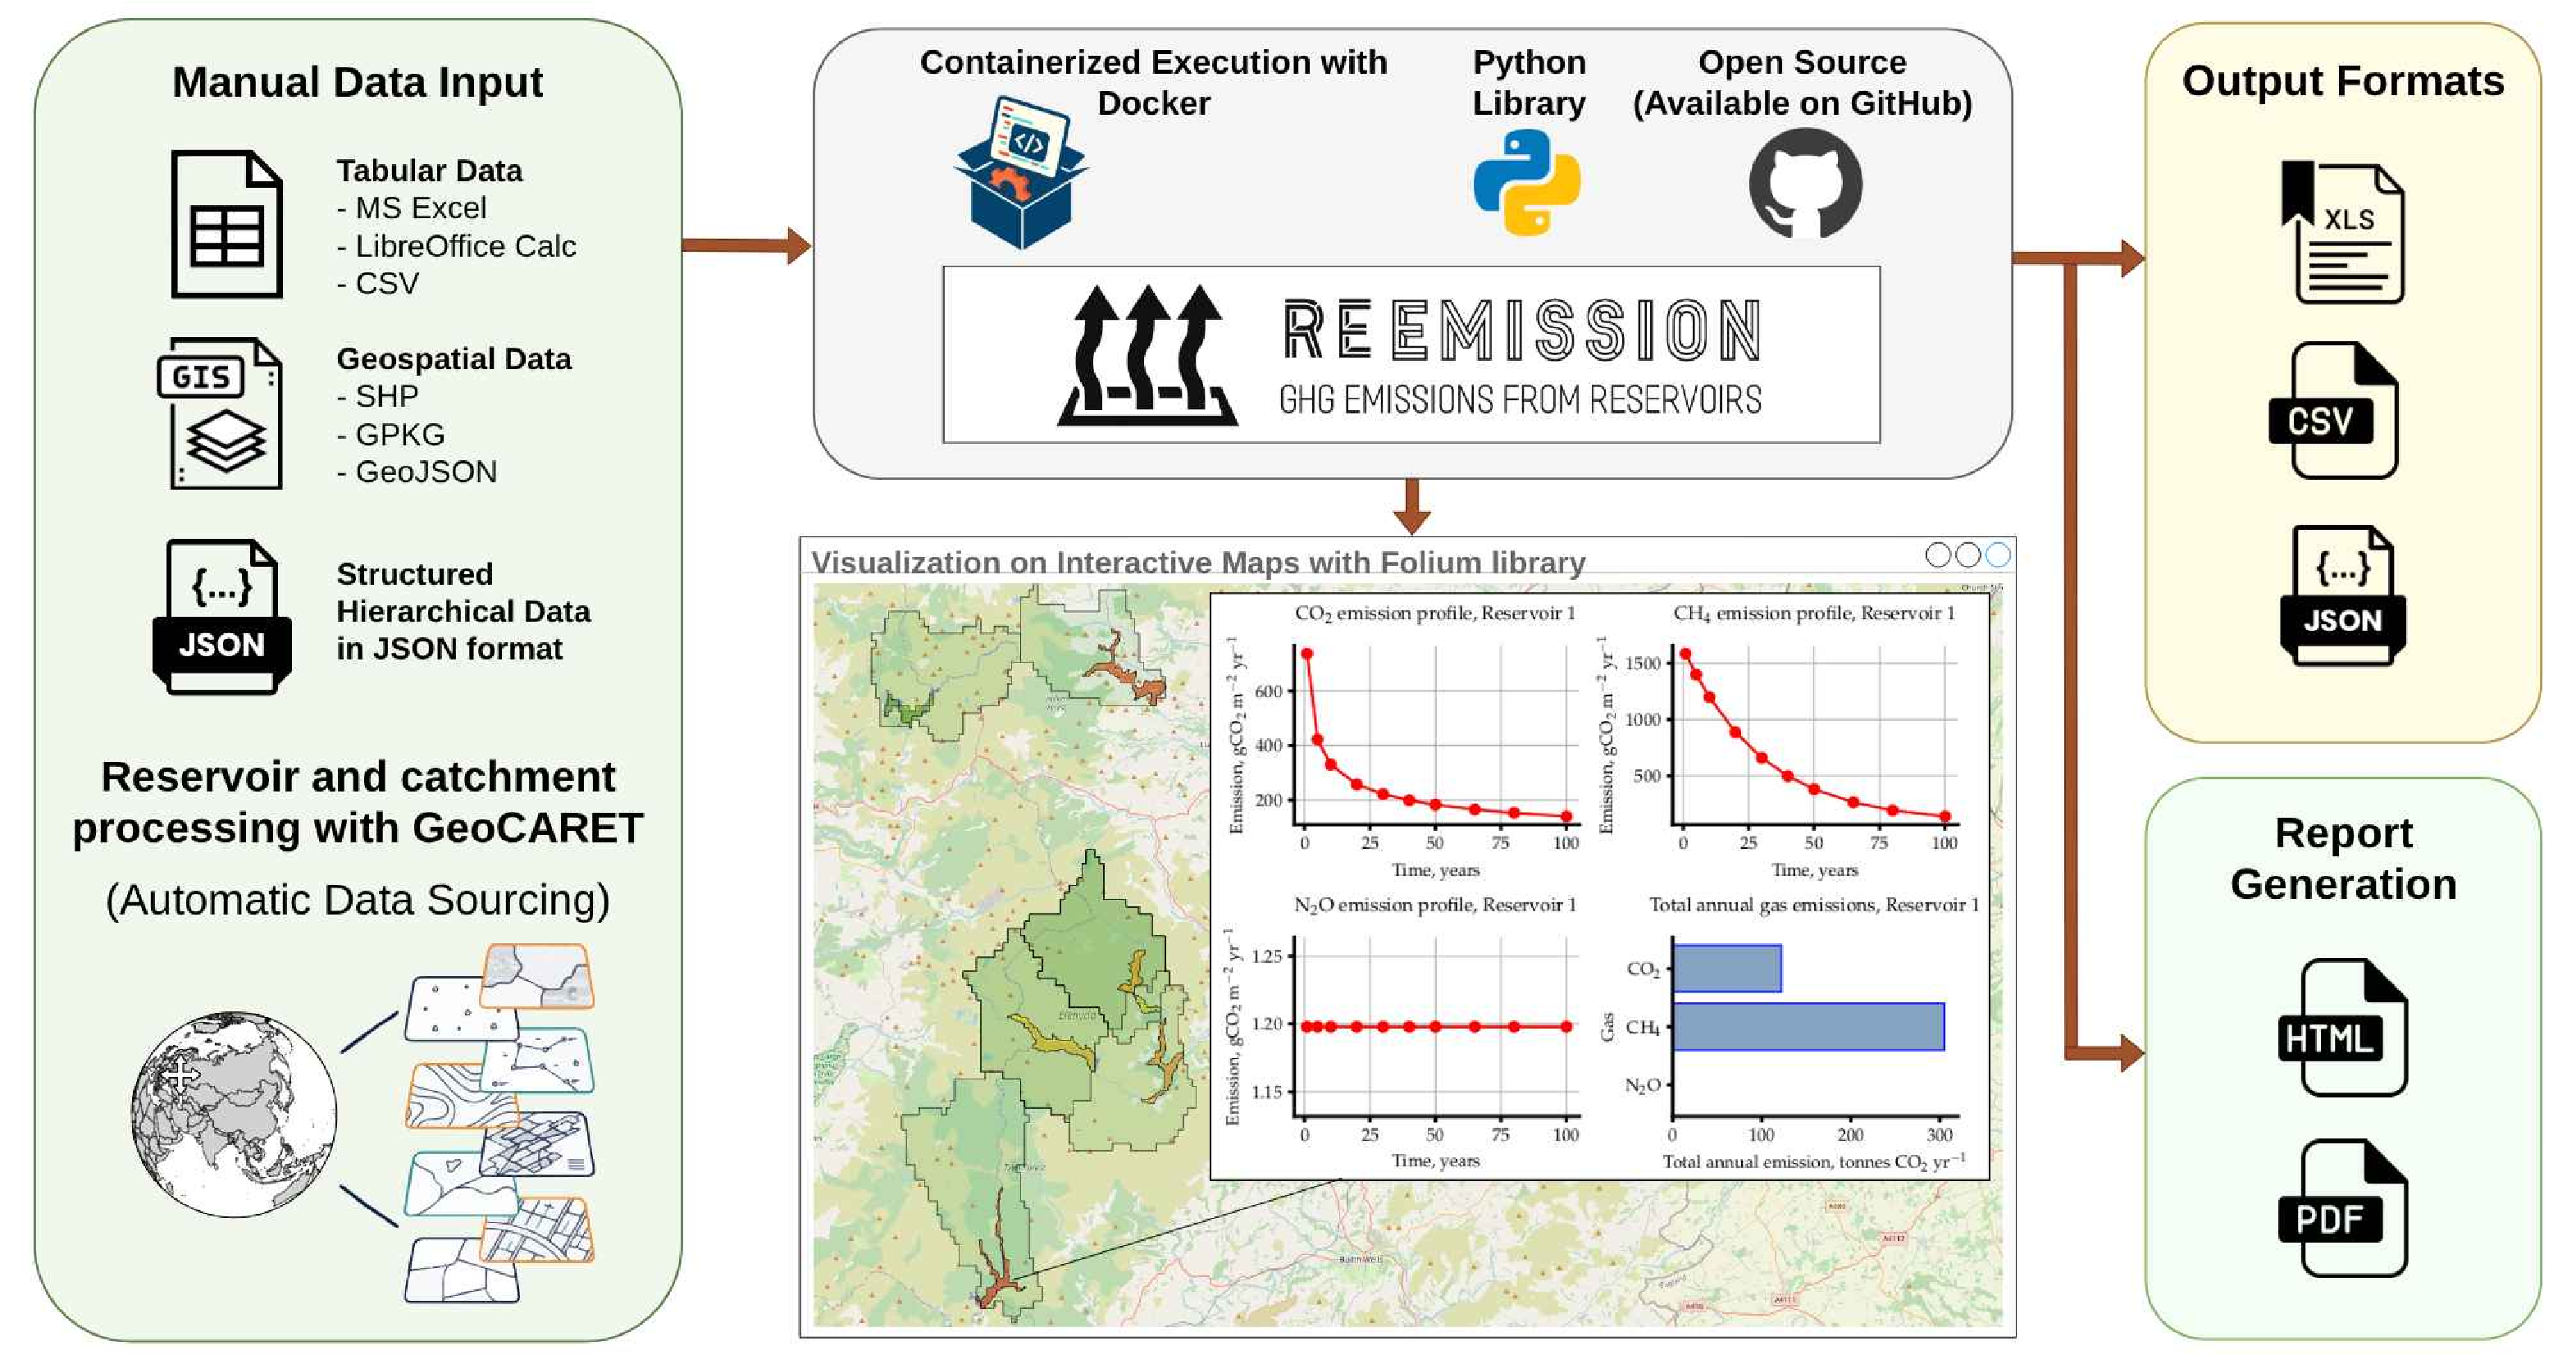
\includegraphics[width=1\textwidth]{figures/graphical_abstract_new_rev1.drawio_11zon.pdf}
\end{graphicalabstract}

%%Research highlights - OLD
%\begin{highlights}
%\item Command line tool and a Python library for calculating reservoir emissions.
%\item Configurable calculation and visualization options.
%\item Integrates with \acs{GIS}-based catchment and reservoir delineation tool.
 %%\item Automates emission calculations from multiple reservoirs.
%\item Supports multiple output and report formats.
%\item Applications in the United Kingdom and Myanmar highlight Re-Emission's features.
%\end{highlights}

\begin{highlights}
\item Re-Emission is a command-line tool and Python library for reservoir GHG analysis.
\item It automates GHG emission estimates across multiple reservoir systems.
%\item The tool offers configurable calculation and visualization of emission results.
\item It integrates with a GIS-based tool for reservoir and catchment analysis.
\item It supports multiple output and report formats and configuration options.
\item Case studies in the United Kingdom and Myanmar highlight Re-Emission's features.
\end{highlights}

%% Keywords
\begin{keyword}
automated assessments \sep greenhouse gas emissions \sep modelling library \sep free open source
%% keywords here, in the form: keyword \sep keyword
%% PACS codes here, in the form: \PACS code \sep code
%% MSC codes here, in the form: \MSC code \sep code
%% or \MSC[2008] code \sep code (2000 is the default)
\end{keyword}

\end{frontmatter}

\section{Introduction}
\label{sec:introduction}

Reservoirs are increasingly recognized as significant sources of biogenic \ac{GHG} emissions~\citep{Barros2011}, particularly in low-altitude tropical regions where emission intensities of hydroelectric dams (e.g., kg~CO$_{2e}$\,MWh$^{-1}$) may exceed those of fossil fuel power plants~\citep{Fearnside2002}. 
These emissions arise from the decomposition of organic matter that was either flooded during reservoir construction, transported into the reservoir by riverine runoff, or produced in situ through processes such as algal growth~\citep{Louis2000}.
Recent estimates suggest that existing reservoirs contribute approximately 5.2\% of global anthropogenic \ac{CH4} emissions and 0.2\% of \ac{CO2} emissions, together accounting for 1-2\% of total anthropogenic \ac{GHG} emissions~\citep{Soued2022}.
Continued and planned investments in new reservoir infrastructure are projected to exacerbate these emissions, hindering progress toward achieving the climate goals of the Paris Agreement.

With more than 3,700 new hydroelectric dams planned worldwide~\citep{Zarfl2015}, potentially contributing an additional 400\,MtCO$_{2e}$ per year~\citep{janus2025planning}, the sector’s total emissions are expected to rise markedly, even when accounting for uncertainties regarding which projects will be realized and their individual emissions.
Projections for planned reservoir investments in sectors such as flood control and water supply are less well documented but are also likely to be substantial, driven by efforts to enhance the resilience of water resources to climatic uncertainty~\citep{ipcc2018, Sarkodie2022}.
Given the potentially high areal \ac{GHG} fluxes from reservoirs, rigorous emission estimation is required both for planned reservoirs -- to inform low-carbon expansion strategies -- and for existing ones -- to improve the accuracy of global \ac{GHG} inventories and assess their climate impacts.
This highlights the need for practical, openly licensed tools that support routine emission estimation and foster continual development and broad uptake across the sector.

%Although several estimates of the total number and total area of reservoirs worldwide have been constructed, contemporary advances in remote sensing and global hydrological mapping have considerably increased our understanding of their true extent and distribution.
%\citet{Downing2006} estimated the number of impoundments globally at 515,149 with a total area of 258,570~km$^2$
%More recent studies provide significantly higher estimates: $\sim$2.8 million reservoirs with a total area of $\sim$530,000~km$^2$~\cite{Mulligan2020} and $\sim$2.5 million with $\sim$642,000~km$^2$ total surface area~\cite{LehnerMessager2023}. 
%All of the above figures are considerably larger than those reported in global dam databases such as \acs{FHReD}~\cite{Zarfl2015FHReD} ($\sim$40,000), \acs{GOOD2}~\cite{Mulligan2021GOOD2} ($\sim$38,667), or \acs{ICOLD}~\cite{ICOLD2020} ($\sim$58,700). 
%These discrepancies stem largely from improved satellite imagery and detection methods that can now identify millions of small and previously undocumented reservoirs.
%Given the likely exclusion of numerous existing reservoirs with unquantified atmospheric impacts, current global emission estimates may require reassessment to account for these new contributions.

Several studies have addressed the methodological challenges of quantifying reservoir emissions and have provided estimates of \ac{GHG} emissions from existing reservoirs at both global~\citep{Barros2011, Soued2022, Deemer2016, Prairie2018, Harrison2021} and regional scales~\citep{Hidrovo2017, Rasanen2018, Almeida2019, Hansen2022}. 
These studies have shown that reservoir emissions are shaped by a complex interplay of hydro-morphological, edaphic, climatic, and land-use characteristics of reservoirs and their catchments~\citep{Deemer2016, Prairie2021} requiring multi-variate emission models.
Meanwhile, current global assessments, including the most recent~\citep{Harrison2021, Soued2022}, have relied on empirical flux approximations derived from a limited number of measured sites, rather than on the direct application of spatially explicit emission models to individual reservoirs.
While these approaches have been instrumental in advancing our understanding of global reservoir emissions, they offer limited capacity to capture the variability in fluxes arising from site-specific environmental conditions and reservoir characteristics -- an aspect that remains crucial for informed reservoir planning~\citep{janus2025planning} and for further improvement of global emission estimates.
A major barrier to moving beyond Tier~1 \acfp{EF} and upscaling is the lack of software capable of applying spatially explicit emission models to estimate reservoir emissions at national, regional, and global scales.

%Moreover, s the measurement data used for upscaling are biased toward large, deep hydroelectric reservoirs~\citep{Hansen2022} and underrepresent smaller, shallower systems rich in organic matter that favour methane production~\citep{Malerba2022, WANG2025123441, SHI2025}, recent global \acp{EF}~\citep{Harrison2021, Soued2022} likely underestimate emissions from small reservoirs, such as those used for irrigation.

The most comprehensive and widely recognized model for estimating reservoir \ac{GHG} emissions is the G-res model~\citep{Prairie2017b, Prairie2021}, which provides spatially explicit estimates of both gross and net emissions by accounting for anthropogenic and natural sources, as well as a broad range of climatic, hydro-morphological, edaphic, and land-use drivers.
G-res is accessible via the publicly available web-based G-res Tool~\citep{prairie2017gres}. %, which offers free assessments for non-commercial users, while commercial applications require validation by the G-res team for a fixed fee.
While easy to use and supported by a distinguished expert committee, the G-res Tool (v3.31) is primarily designed for single-reservoir assessments.
It enables retrieval of selected input parameters from global geospatial datasets via Google Earth Engine~\cite{Gorelick2017}; however, because this process must be performed manually, its capability to support multi-reservoir analyses is limited.
Furthermore, as the tool is closed-source, it cannot be freely modified or extended by users, which constrains its adaptability for customized workflows and advanced applications, including stochastic modelling, strategic planning, and the integration of custom sub-models.

%The development of a free open-source alternative could offer the following benefits: (i) direct use of complete emission models, instead of upscaling methods, may help removing potential biases in global estimates and improve the accuracy of emission estimates for individual reservoirs, (ii) they will enable a more precise estimation of emissions from reservoirs whose characteristics fall outside the range of values represented in the measurement data sets (iii) they will enable an easier transition from Tier~1 may not be adequate to represent emission rates in different regions as well as different reservoir morphologies into more methodological methods without imposing significant overheads in terms of costs and time, (iv) 

%This upscaling approach assumes that areal fluxes for a given gas or emission pathway remain constant within a specific area of interest, such as a latitude~\cite{Harrison2021} or climatic zone~\cite{Soued2022} and does not take into account the effects of the multitude of emission drivers on emission rates~\citep{Deemer2016, Prairie2021} that vary widely across the diverse reservoir morphologies and their geographic settings.
%upscaling emissions from a small number of reservoirs with measured emissions to global emissions by 
%Precision due to identification of reservoir area and locations and estimation methods - ever growing numbers 
%However, these databases a rather high estimate for total area\,km$^2$ -- ~480,000 in GOOD2.
%Shows that missing data is for small reservoirs ...

Here, we introduce \textit{Re-Emission} -- a free open-source library written in Python for estimating, visualizing, and reporting \ac{GHG} emissions from reservoirs. 
Owing to its open-source design, \textit{Re-Emission} allows modifications and extensions to incorporate new datasets, implement new emission models and sub-models, adjust model parameters, and accommodate other project-specific requirements, enabling the development of custom reservoir emission analyses.
Implemented in Python -- a widely used language in the scientific and engineering communities -- \textit{Re-Emission} can be readily introduced into broader modelling or planning frameworks. 
Through integration with the upstream reservoir and catchment processing tool GeoCARET~\citep{heettool}, it enables automated estimation of regional- to national-scale emission inventories using spatially explicit models, thus advancing beyond Tier~1 approximations -- in line with recommendations from the IPCC~\citep{IPCC2019}.
Since the G-res implementation in \textit{Re-Emission} has been validated against the published G-res Tool~\citep{prairie2017gres, Prairie2021} (v3.31), the software can be reliably used for practical assessments of reservoir \ac{GHG} emissions.

This paper is structured as follows.
First, we review the availability of software for reservoir emission modelling and position \textit{Re-Emission} within this broader landscape.
Second, we provide a high-level overview of the software architecture, highlighting its main components and capabilities.
Third, we outline key features of the tool, including its dual use as a Python library for simulating reservoir emissions and as an implementation of existing models. 
We describe the basic usage of the Python library, available configuration options, supported input and output formats, and emission-reporting functionalities.
Fourth, we demonstrate an optional execution method via Docker and integration with GeoCARET~\cite{heettool} -- a command-line tool written in Python for delineating and analysing catchments and reservoirs using Google Earth Engine's cloud computing platform and assets~\cite{Gorelick2017}. 
Finally, we present two use cases that illustrate the practical utility of \textit{Re-Emission} in real-world applications, estimating emissions from approximately 250 reservoirs in Myanmar and the United Kingdom.

\section{Availability of software for reservoir emission modelling}
\label{subsec:software_and_code}

Despite growing research interest and practical relevance (see the historical review in Supplementary Materials), software tools for reservoir \ac{GHG} emission modelling remain scarce.
Only a few modelling frameworks are accompanied by openly available tools that can be readily applied by practitioners.

Among currently available solutions, the G-res Tool~\cite{Prairie2017b,prairie2017gres} -- v3.31 at the time of writing -- constitutes the most advanced and operationally mature implementation currently accessible to practitioners.
It provides a web-based interface designed for hydropower developers, consultants, and stakeholders, implementing the G-res empirical regression model to estimate net anthropogenic \ac{GHG} emissions from reservoirs using widely available inputs without requiring field measurements~\citep{Prairie2021}. 
The tool supports allocation of emissions to reservoir services and includes modules to account for emissions associated with construction and infrastructure.
%Validation of tool results is required for public disclosure in commercial applications, which lends credibility and ensures appropriate use of the methodology.
The G-res Tool is available at no cost for non-commercial use, while commercial users are subject to a review and validation process by the G-res Expert Committee, incurring a fixed fee.
In addition, the G-res team offers further paid assessment services (e.g. ``Results Report'' and ``Full Report'' options) that provide certified emission estimates and detailed reporting ~\citep{prairie2017gres}.

Mechanistic (process-based) models such as CE-QUAL-W2~\citep{Berger2014}, LAKE~2.0~\citep{Lomov2024, Stepanenko2016}, and the \ac{EFDC} model~\citep{hamrick1992, SHI2025} are generally embedded within broader environmental or hydrodynamic modelling frameworks.
These models explicitly simulate the thermal and biogeochemical dynamics governing \ac{GHG} production and transport, offering higher process fidelity but reduced suitability for routine or large-scale assessments.
Their accessibility also varies: \ac{EFDC} is distributed as proprietary Windows executables without source code or official support, whereas LAKE~2.0, though open-source and cross-platform, is available only upon request rather than through a public repository.
By contrast, CE-QUAL-W2 is freely available under the MIT license and has been successfully applied in reservoir emission studies~\cite{Berger2014, Wu2022}.
Several other open-source lake models -- such as Flake, GLM, GOTM, Simstrat, and MyLake -- are available and can be run individually or collectively via the LakeEnsemblR R package for ensemble lake modelling~\cite{Moore2021}.
These lake models can, in principle, be extended to describe emission processes, such as those published in \cite{Soued2020exp}, although such implementations are not yet broadly accessible to the scientific community.

The limited availability of free, open, extensible and customizable software for reservoir \ac{GHG} emission assessment underscore a persistent gap between scientific model development and practical implementation.
Bridging this gap is essential for translating research advances into operational tools and incorporating emission models into broader frameworks for low-carbon reservoir planning and reservoir assessments -- many of which still rely on Tier~1 approaches~\cite{Almeida2019, Carlino2024, Tangi2024}.
Developing open-source, modular software ecosystems represents a critical step toward enabling such integration. % at regional to global scales.

\section{The \emph{Re-Emission} package}
\label{sec:reemission}

Re-Emission is a free, open-source software package written in Python and supplied under the GNU General Public License v3.0, designed to be used both as a library and a \acf{CLI} tool. It serves two main purposes.

First, it provides an openly available and documented collection of Python classes that form a foundation for experimenting with existing reservoir emission models and developing new extensions.
The software is structured around the G-res framework, which offers a blueprint for estimating CO$_2$ and CH$_4$ emissions through multiple pathways and introduces the methodology for estimating emissions attributable solely to reservoir creation, i.e. ``What Does the Atmosphere See?''~\citep{Prairie2018}.
Following the G-res framework, Re-Emission reports both gross and net emissions integrated over a 100-year time horizon, as well as annual temporal profiles starting from the impoundment year.
The hydro-morphological, edaphic, climatic, and land-use emission drivers are defined on catchment and reservoir levels and instantiated from input-data using respective \texttt{Catchment} and \texttt{Reservoir} classes.
By adopting the conceptual and structural design of G-res, Re-Emission enables researchers to extend the framework with new emission models and submodels without having to develop their own interfaces or reimplement existing formulations.

Second, Re-Emission provides a free and open-source implementation of the state-of-the-art G-res model~\citep{Prairie2021}, two reservoir phosphorus retention models~\citep{larsen1976, Maavara2015}, the nitrogen and phosphorus land export model of \citet{McDowell2020}, and two nitrous oxide emission models~\citep{Maavara2019, Akbarzadeh2019}.
Our implementation accurately reproduces the behaviour of the G-res Tool v3.31 -- the web-based interface implementation of the G-res model -- when using equivalent phosphorus retention and terrestrial export submodels (see Emission Model Validation and Supplementary Results).
The nitrous oxide emission models are currently unvalidated and therefore considered experimental.
Model parameters can be configured via external configuration files or adjusted dynamically at runtime, supporting applications such as sensitivity analysis and calibration.
The implementation also supports batch processing of multiple reservoirs, and emission reporting and visualization in different formats.

Practical examples of these capabilities are illustrated through a set of Jupyter Notebooks~\cite{Kluyver2016jupyter} and an accompanying demo (see \emph{Software Availability}).
Additional details on the software architecture and functionality are presented in the following sections.

\subsection{Design}
\label{subsec:design}

\begin{figure}[ht]
    \centering
    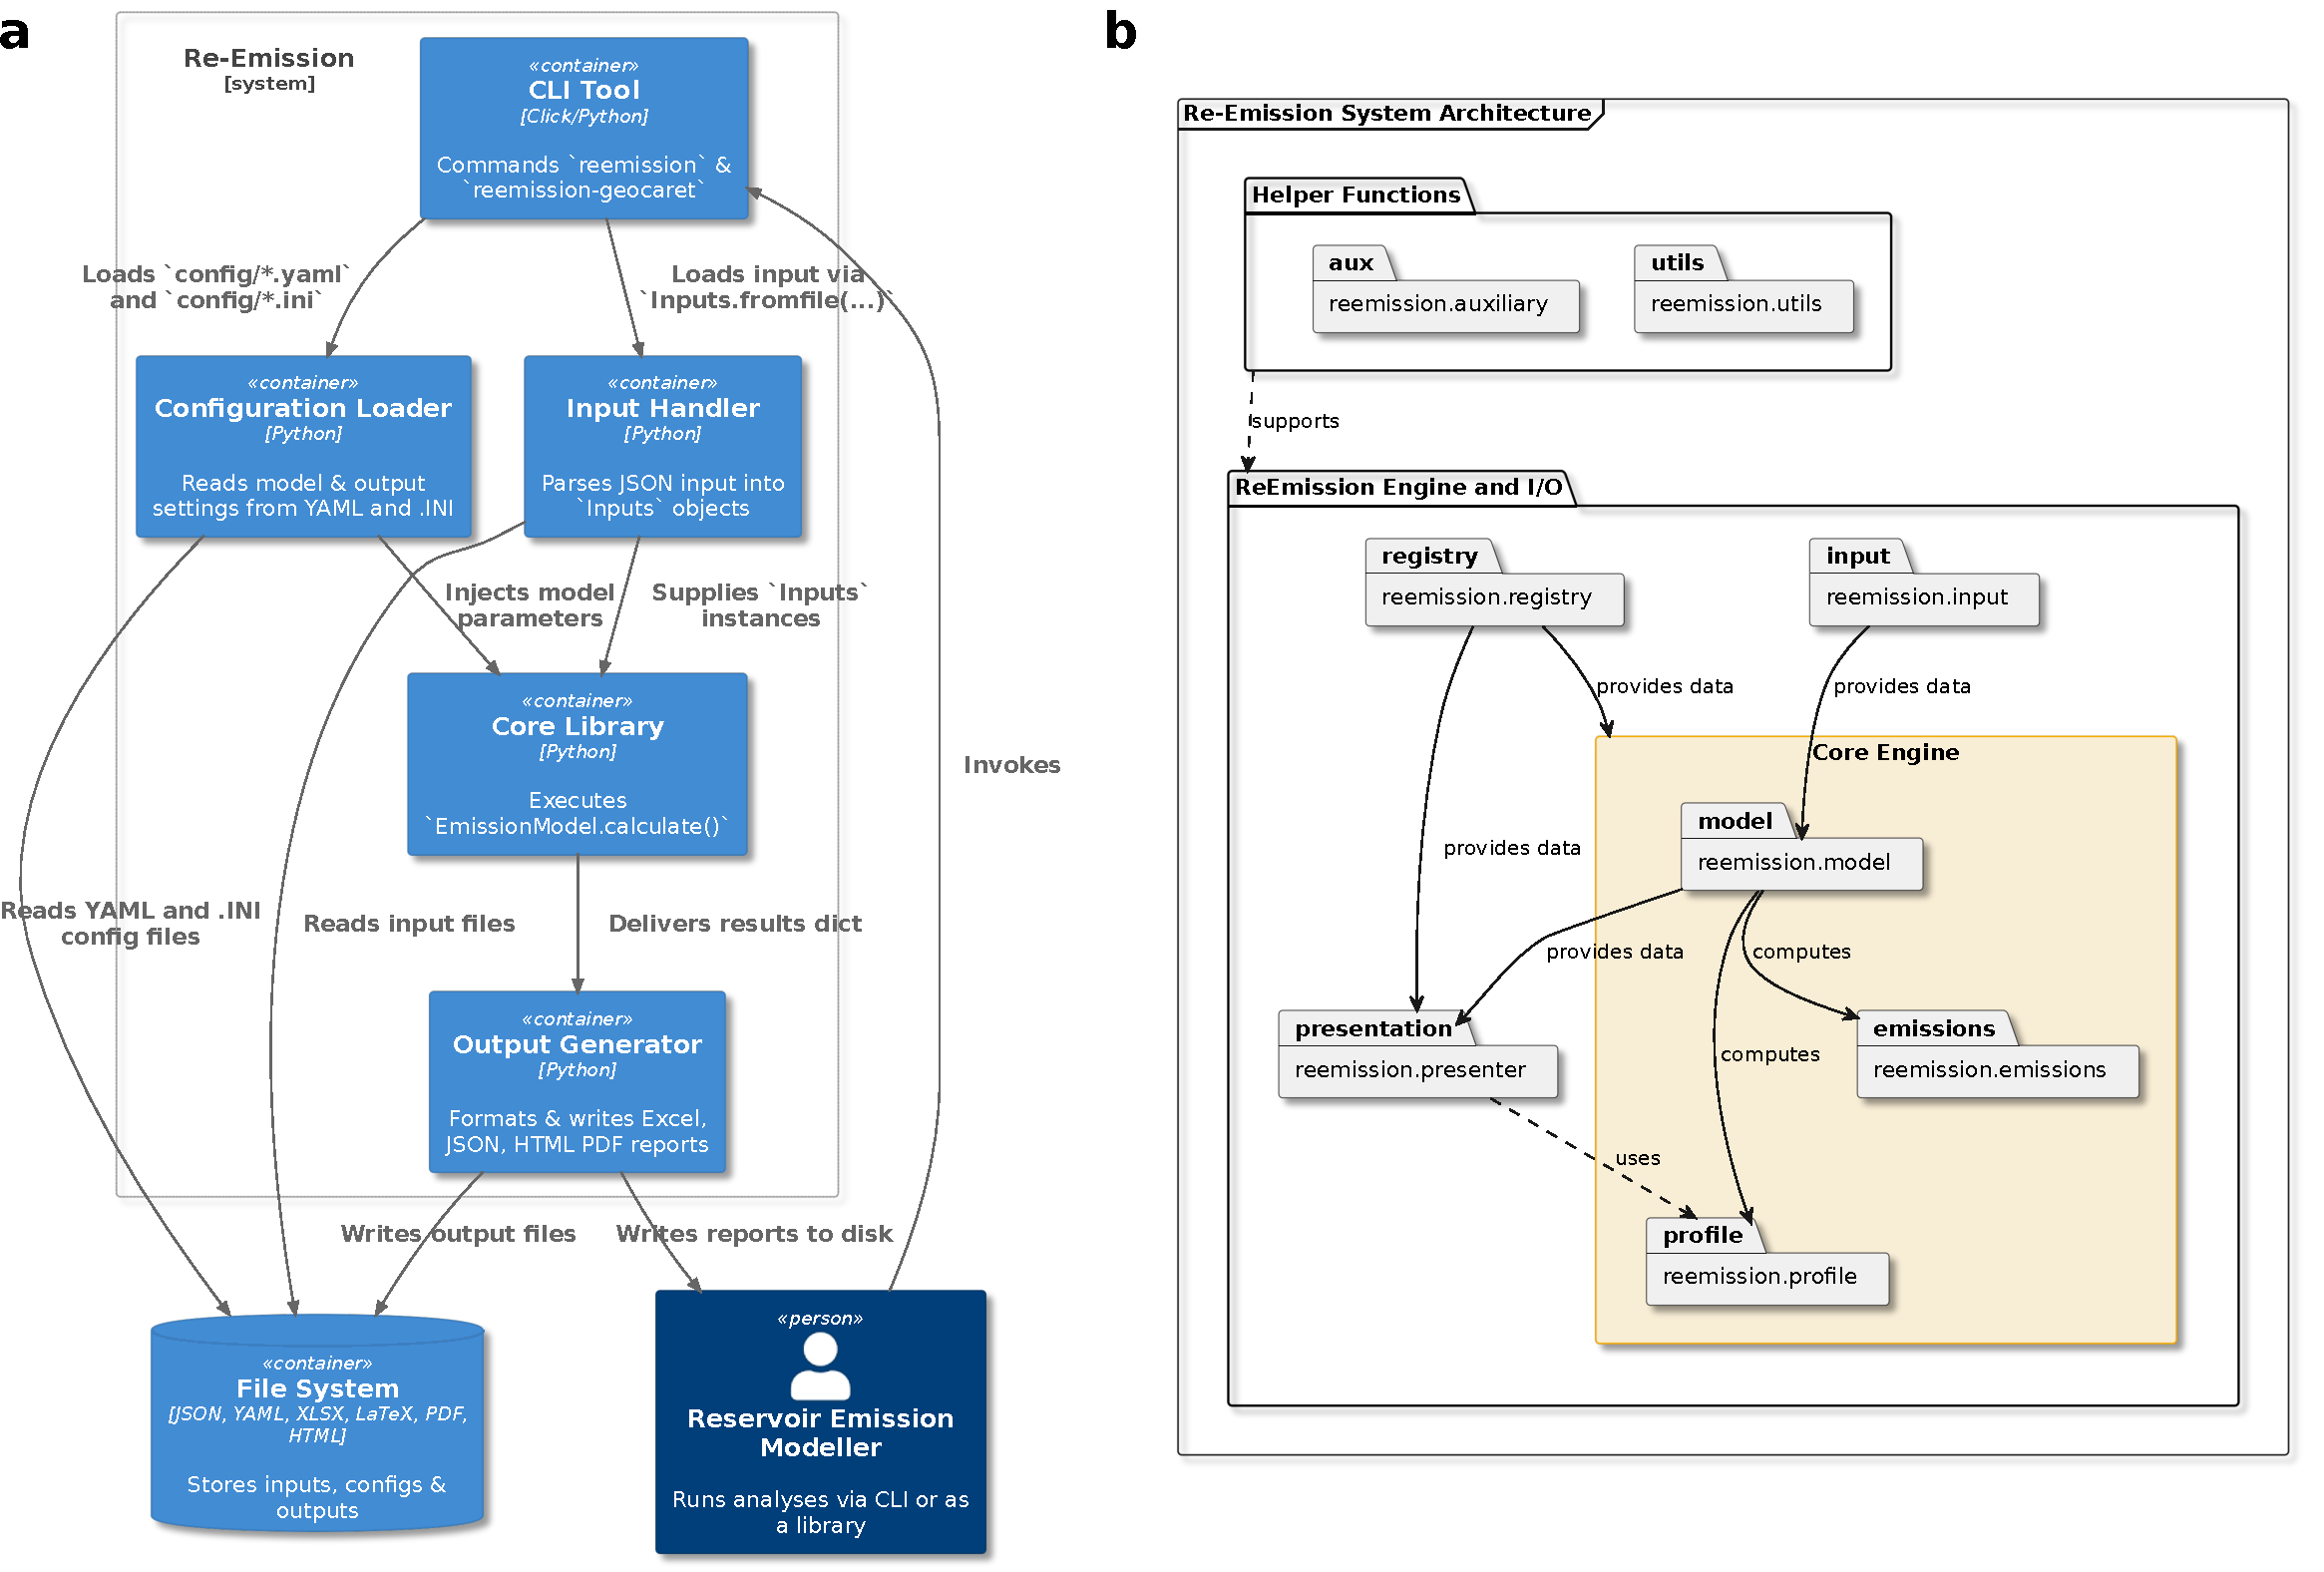
\includegraphics[width=0.99\textwidth]{figures/high_level_achitecture.pdf}
	\caption{Architecture of \textit{Re-Emission}. \textbf{a}, Container-level interactions showing key components, their functionalities, and data flow between system elements. Users can interact with the \acf{CLI} or Python library to load configuration parameters and input data, run the core emission models, and generate reports in multiple formats (Excel, JSON, PDF, HTML). Configuration files specify model parameters and presentation settings for the outputs, while the file system manages input and output storage. \textbf{b}, Package dependency view highlighting the modular structure and inter-package relationships within the system.}
    \label{fig:high_level_archtecture}
\end{figure}

The high-level architecture of the Re-Emission framework is illustrated in Figure~\ref{fig:high_level_archtecture}.
Re-Emission can be used either via a \acf{CLI} or by directly accessing its Core Library components within Python scripts, as shown in Figure~\figref[a]{fig:high_level_archtecture}.
The \ac{CLI} serves as the primary user interface, enabling emission analyses through straightforward commands.
When a command is executed, control is passed to a configuration loader, which parses and validates the user-defined model parameters, execution settings (e.g., selection of submodels), and presentation options (e.g., choice of output variables and associated metadata).
The default configurations specified in YAML and INI files are located in the \vrbbrk{reemission/config/} directory.
The user can additionally override these settings by providing own configuration files and typing the path to the configuration folder in the command line. 
The configuration settings are passed to both the Core Library and the \vrbbrk{reemission.presenter} module (Figure~\figref[b]{fig:high_level_archtecture}).
This design enforces a clear separation between logic (model equations) and data (parameters and inputs).

Input data are provided in JSON format and include reservoir, catchment, and climatic variables. 
These are read by \vrbbrk{reemission.input} and converted into a strongly typed \vrbbrk{Inputs} object used by the emission model.
Input data can be compiled manually from various data sources or generated automatically through upstream tools such as GeoCARET~\cite{heettool}, with which Re-Emission integrates (see Section~\ref{sec:integration}).
Upon completion of a model run, outputs are passed to a reporting engine that generates results in multiple formats, including Excel workbooks (XLSX), structured JSON files, as well as HTML and PDF reports.
Presentation functionality is handled by \vrbbrk{reemission.presenter}, which collates inputs, outputs, and intermediate variables from \vrbbrk{reemission.model} and \vrbbrk{reemission.profile}.
This enables both textual and graphical visualisations of the simulation outputs.
The loading, modification, and reuse of configuration files are managed by the \vrbbrk{reemission.registry} module.
%e cumulative reservoir emissions over time, based on each reservoirs' impoundment dates and their respective emission decay rates. 
% % -- such as regression coefficients, pre-impoundment emissions, and nutrient exports from land -- such as choice of submodels
%The input data and configuration settings are then routed into the Core Library highlighted in Figure~\figref[b]{fig:high_level_archtecture} by a lemon yellow rectangle. 
%The Core Library comprises the emission model, which runs the analysis using selected emission models and passes the results to \vrbbrk{reemission.presenter}. 

\begin{figure}[ht]
    \centering
    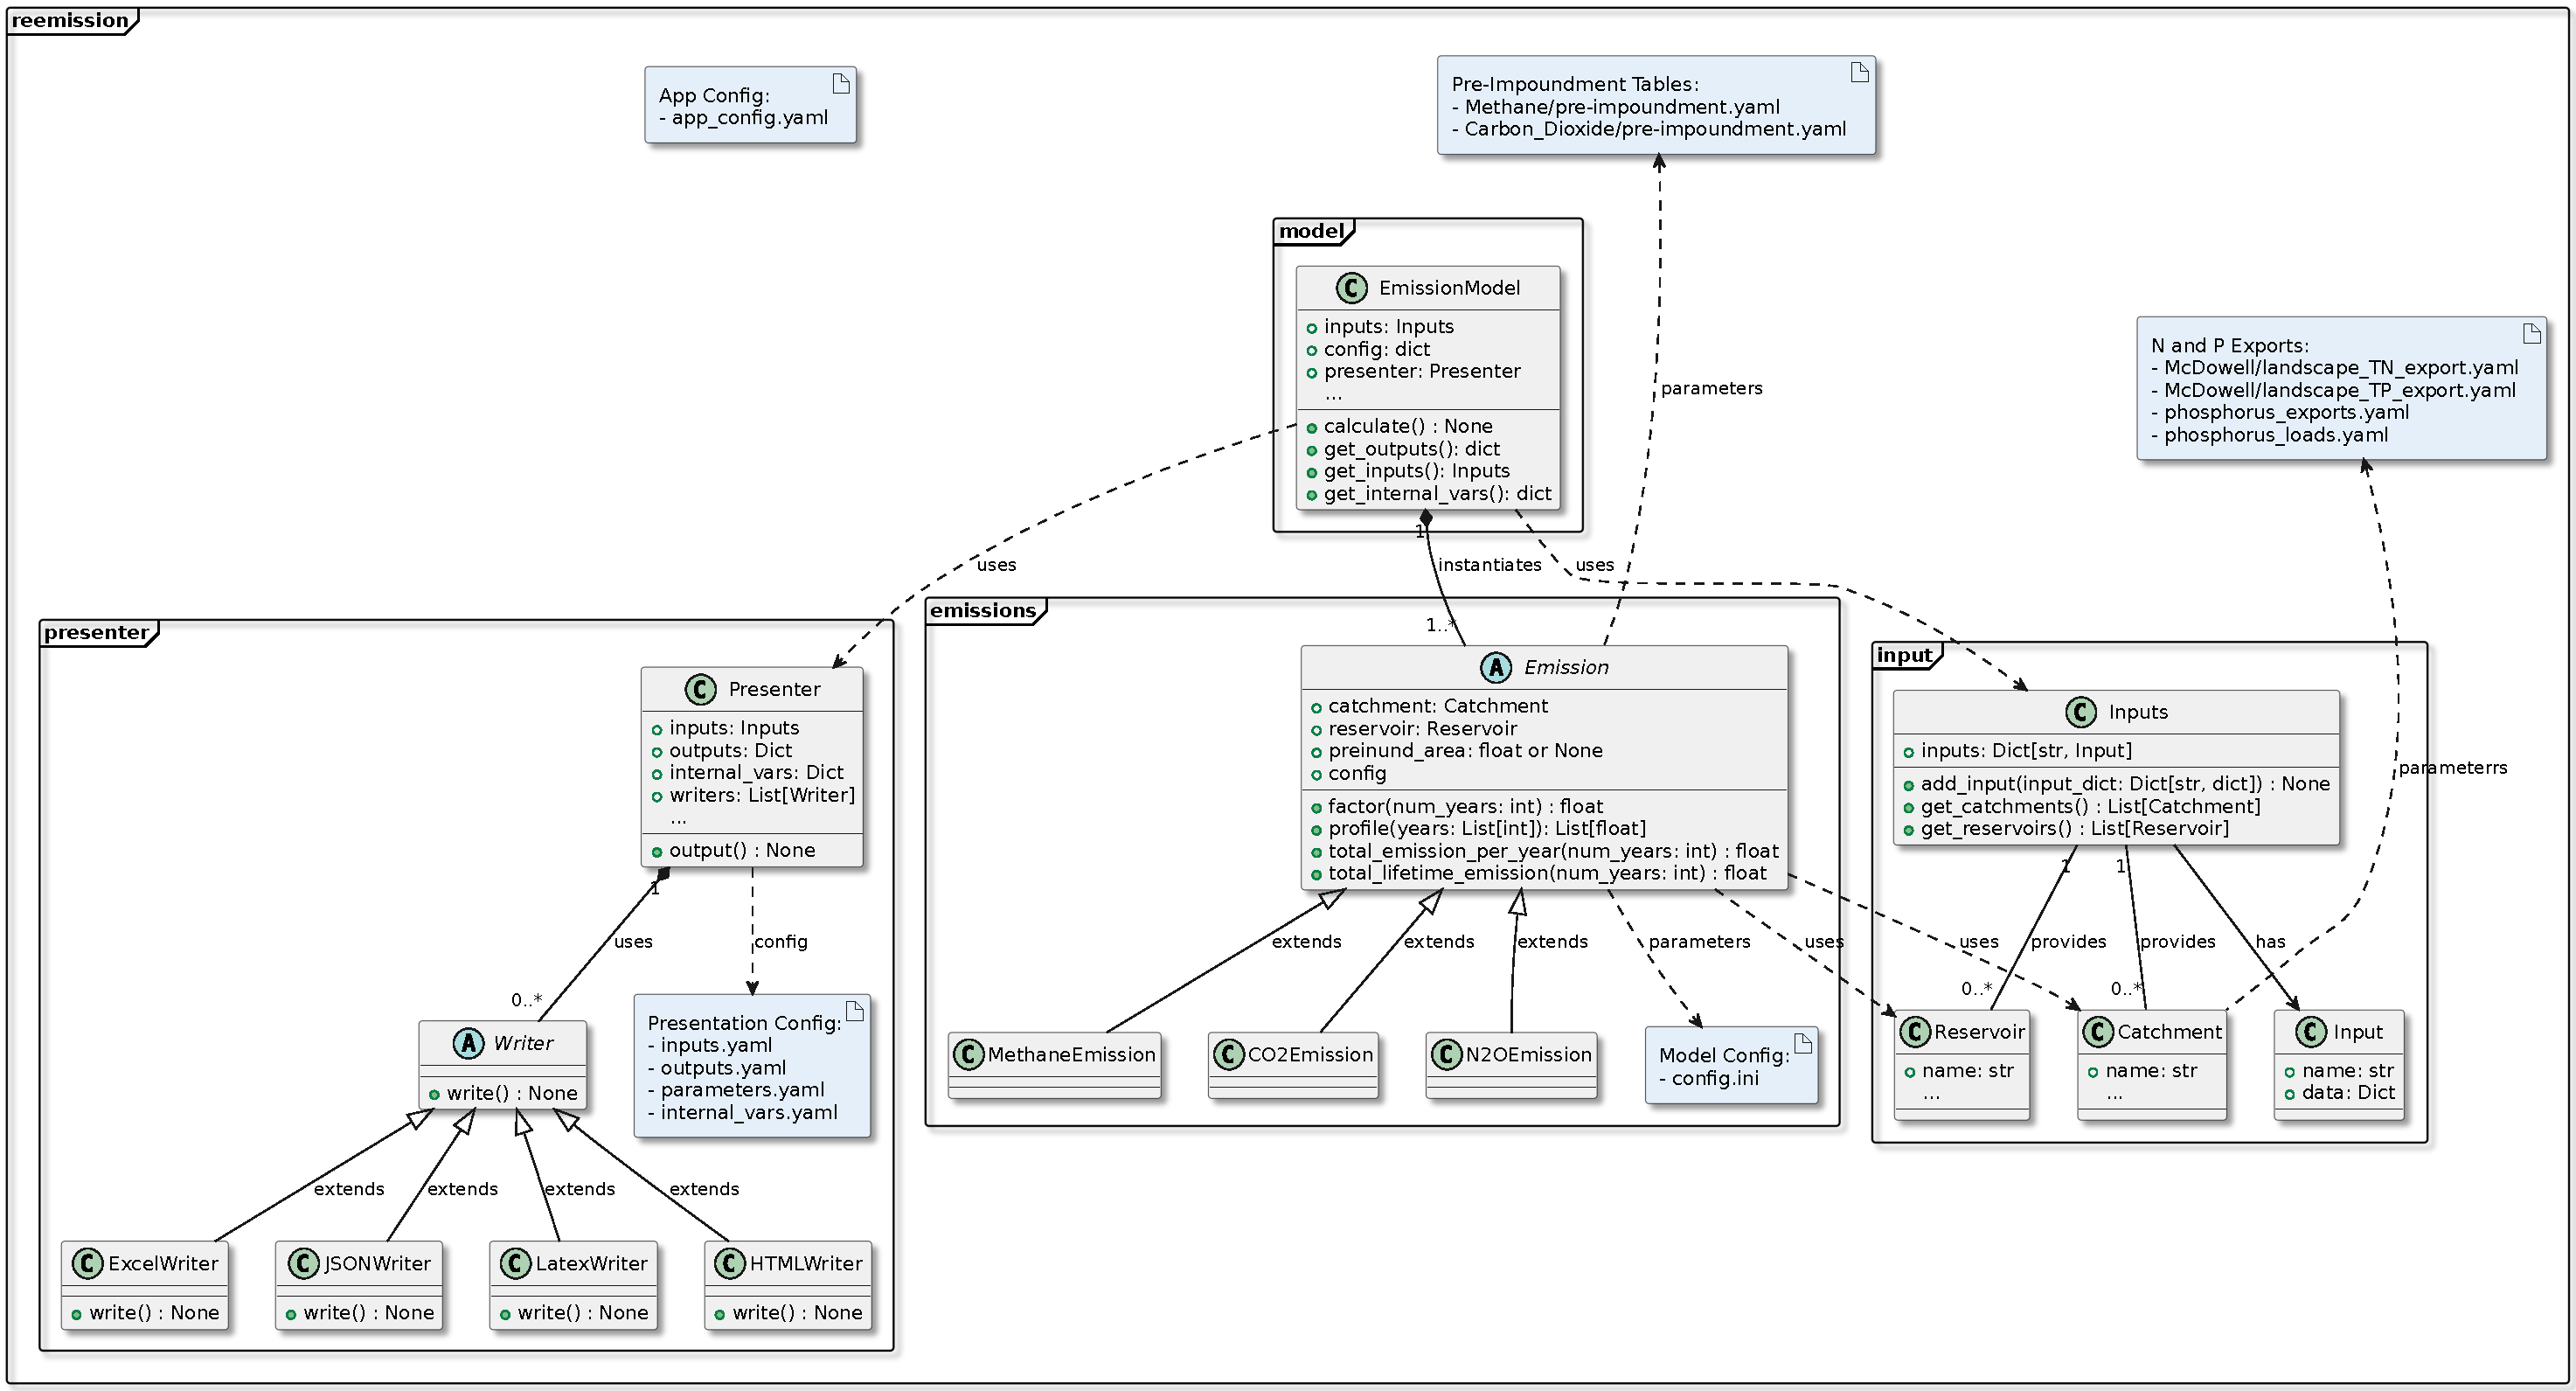
\includegraphics[width=0.99\textwidth]{figures/high_level_uml2.pdf}
	\caption{UML class diagram of \textit{Re-Emission}, illustrating key classes and their relationships. Core components include \texttt{EmissionModel}, \texttt{Reservoir}, \texttt{Catchment}, \texttt{Emission}, \texttt{Inputs}, and \texttt{Presenter}, with abstract interfaces used to enforce modularity and extensibility.}
    \label{fig:high_level_uml}
\end{figure}

A more detailed representation of the internal structure and inter-class relationships is shown in the UML class diagram in Figure~\ref{fig:high_level_uml}.
The \texttt{EmissionModel} class encapsulates the core simulation logic, including the instantiation of \vrbbrk{Reservoir}, \vrbbrk{Catchment}, and \vrbbrk{Emission} objects (e.g., \vrbbrk{MethaneEmission} for CH$_4$), and the subsequent computation of intermediate and output \ac{GHG} variables.
The \vrbbrk{Reservoir} and \vrbbrk{Catchment} objects are provided to the \vrbbrk{EmissionModel} via the \vrbbrk{Inputs} class.
Each \vrbbrk{Emission} object inherits from an abstract \vrbbrk{Emission} base class, which defines four abstract methods that must be implemented by all subclasses.
The \vrbbrk{Presenter} class uses \vrbbrk{Writer} objects to export outputs in different formats.
All \vrbbrk{Writer} objects inherit from an abstract \vrbbrk{Writer} base class that defines a unified interface for generating outputs.
Supported output formats include JSON, XLSX, PDF (via \LaTeX), and HTML.
The \vrbbrk{Reservoir}, \vrbbrk{Catchment}, \vrbbrk{Emission}, and \vrbbrk{Presenter} classes are parameterized via configuration files containing regression coefficients, pre-impoundment emission factors, nutrient export rates, and presentation options specific to the \vrbbrk{Presenter}.
Further details on the internal structure of the \vrbbrk{Reservoir} and \vrbbrk{Catchment} classes, as well as model input representations, are provided in the Appendix in Figure~\ref{fig:river_network_emissions_uml}.

\subsection{Using Re-Emission as a library}
\label{subsec:scripting}

Emission calculations can be performed step by step by first constructing \vrbbrk{Reservoir} and \vrbbrk{Catchment} objects, followed by the instantiation and execution of individual \vrbbrk{Emission} objects (for CO$_2$, CH$_4$, etc.), as shown in Listings~\ref{lst:em_calc_setup} and~\ref{lst:em_calc} in the Appendix.
Alternatively, the \vrbbrk{EmissionModel} class provides a streamlined interface for this process, as illustrated in Listing~\ref{lst:em_calc_file}.
In addition to simplifying the model execution, \vrbbrk{EmissionModel} class enables results to be exported in multiple formats through the \vrbbrk{Presenter} class (see Listing~\ref{lst:em_calc_presentation}).
In both usage modes, the analytical workflow -- excluding result presentation -- follows the algorithmic structure outlined in Algorithm~\ref{alg:reemission}. Input data and model parameters are first read from structured data and configuration files. These inputs are then validated prior to computation. Emissions are subsequently calculated for each reservoir defined in the dataset, and raw results are saved to a JSON output file.

\begin{algorithm}[H]
\caption{Reservoir Emission Estimation}
\label{alg:reemission}
\SetKwInOut{Input}{Input}
\SetKwInOut{Output}{Output}

\AlgoDisplayBlockMarkers

\Input{Input file path (e.g., \texttt{input\_file.json})\\
       Configuration file path (e.g., \texttt{config\_file.yaml})}
\Output{Output file path (e.g., \texttt{output\_file.json})}

\BlankLine
Load input data from \texttt{input\_file.json}\;
\If{input is invalid}{
    Raise error and exit\;
}
Initialize model parameters from configuration file\;
\ForEach{entry in dataset}{
    Instantiate \texttt{Reservoir} and \texttt{Catchment} objects\;
    Instantiate \texttt{CarbonDioxideEmission} and \texttt{MethaneEmission} objects\;
    Estimate annual CO\textsubscript{2} and CH\textsubscript{4} fluxes and flux profiles\;
}
Save results to \texttt{output\_file.json}\;
\end{algorithm}


\subsection{Command-Line Interface}
\label{subsec:cli}

Full \acf{CLI} usage instructions are available by running \vrbbrk{reemission --help} in a terminal or console.
A typical command-line invocation is illustrated in Listing~\ref{lst:em_calc_cli}, where input data are supplied in \vrbbrk{input.json}, and outputs are generated in multiple formats, including PDF, JSON, XLSX, and HTML.
Beyond emission calculation, the \ac{CLI} also supports commands for converting and modifying input datasets.
These capabilities are described further in Section~\ref{sec:integration}, which focuses on integration with upstream reservoir and catchment data processing workflows (see also Listing~\ref{lst:integration_cli}).

\begin{minipage}{0.95\textwidth}
\begin{lstlisting}[language=bash, label={lst:em_calc_cli}, caption={Re-Emission \ac{CLI}: Emission calculations using input.json as the source of input data.}]
> reemission calculate 
    input.json
    -o output.pdf -o output.json -o output.xlsx  -o output.html
    --author "John Smith" 
    --title  "Reservoir Emissions Analysis"
\end{lstlisting}
\end{minipage}

\subsection{Input and output data formats}
\label{subsec:input_output_formats}

The structure of the input and output data is illustrated in Figures~\ref{fig:input_data_format} and~\ref{fig:output_data_format}, respectively.
The input format is fixed and determined by the parameter requirements of the \vrbbrk{Reservoir} and \vrbbrk{Catchment} classes.
In contrast, the structure of the output data is configurable via YAML configuration files.
To improve clarity and readability, the figures show only a representative subset of the full input and output content.
Where data has been truncated, omissions are marked using bold, light-blue text followed by an ellipsis (...).

\begin{figure}[ht]
    \centering
    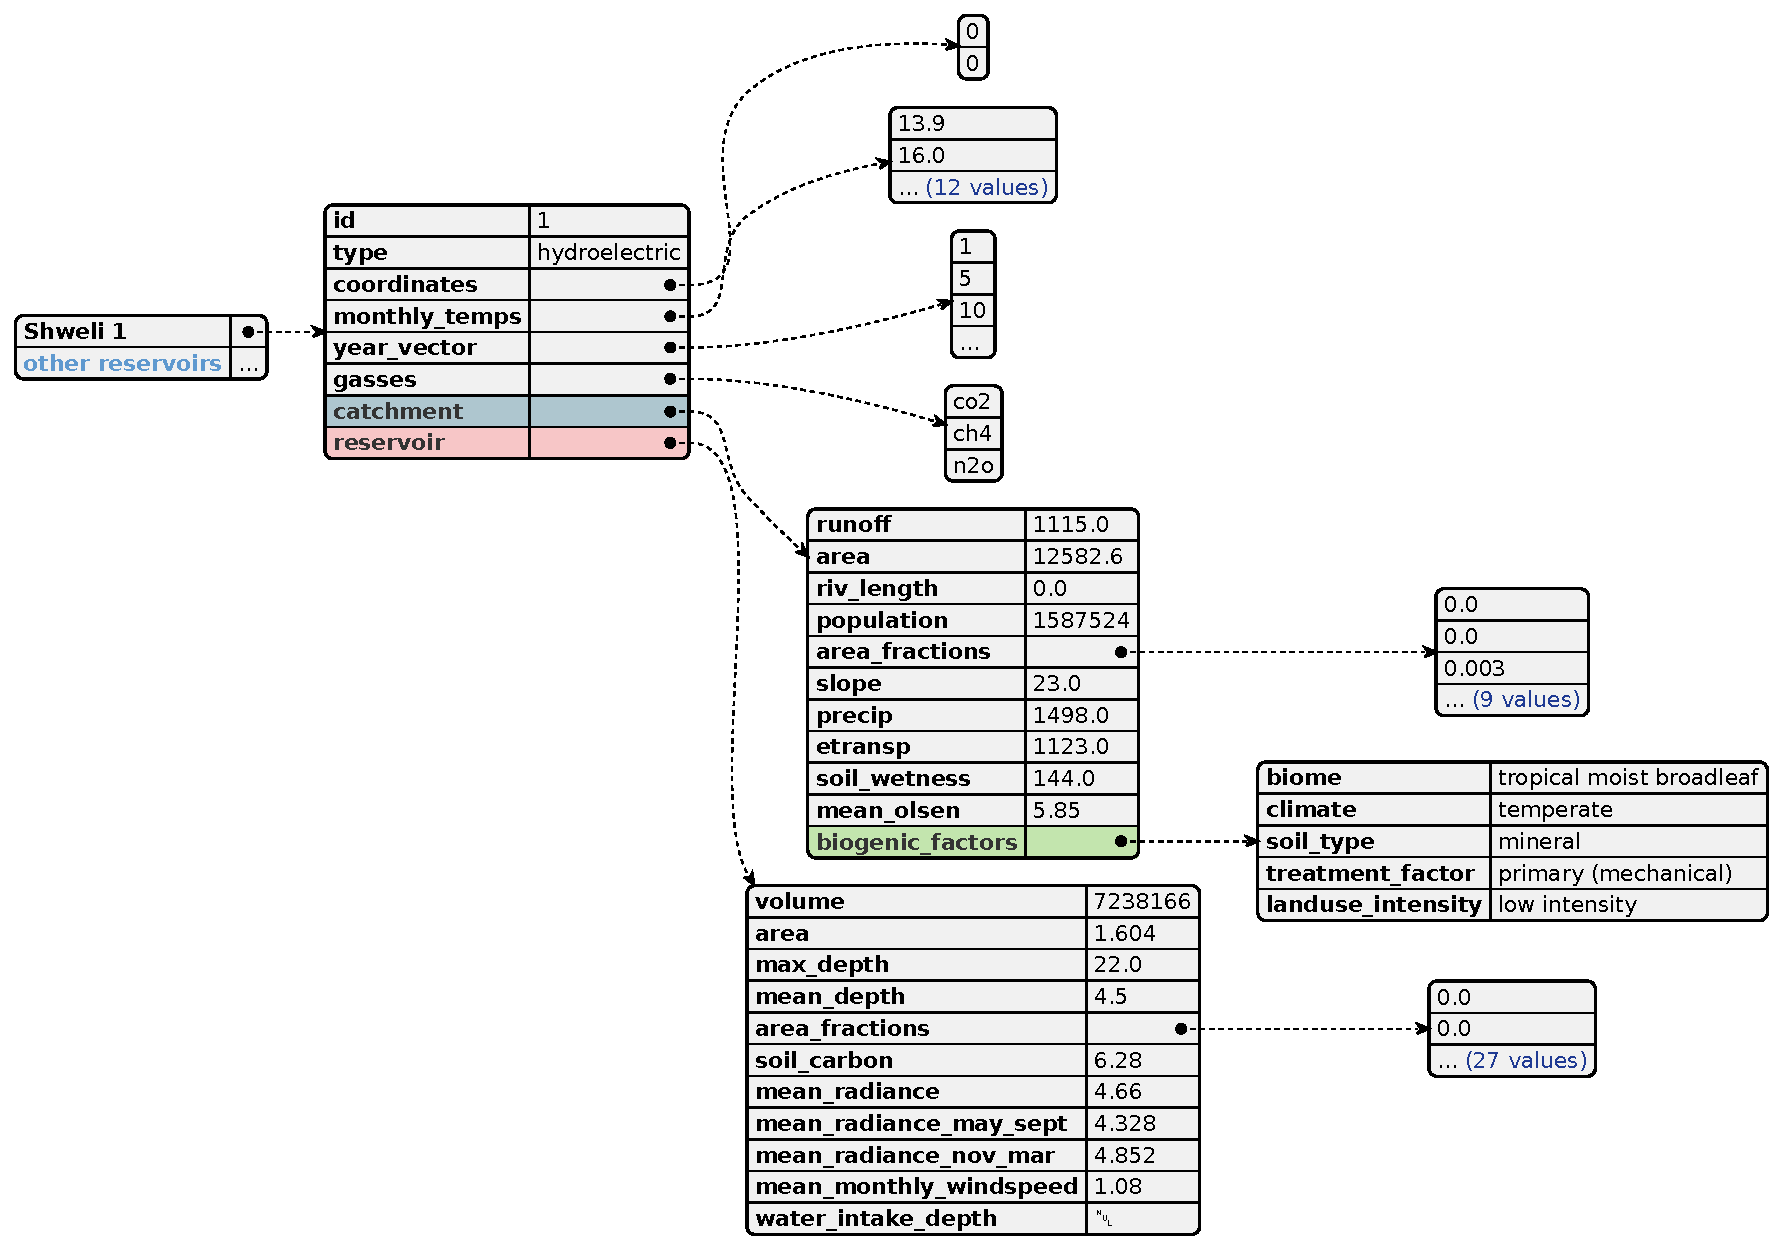
\includegraphics[width=0.75\textwidth]{figures/input_data_json.pdf}
    \caption{Structure of an input JSON file containing example data for a single reservoir. Entries related to catchment and reservoir parameters -- highlighted in steel blue and salmon, respectively -- correspond directly to fields defined in the \vrbbrk{Catchment} and \vrbbrk{Reservoir} classes. Selected values have been truncated for readability, with omissions indicated using light blue font colour followed by an ellipsis.}
    \label{fig:input_data_format}
\end{figure}

\begin{figure}[ht]
    \centering
    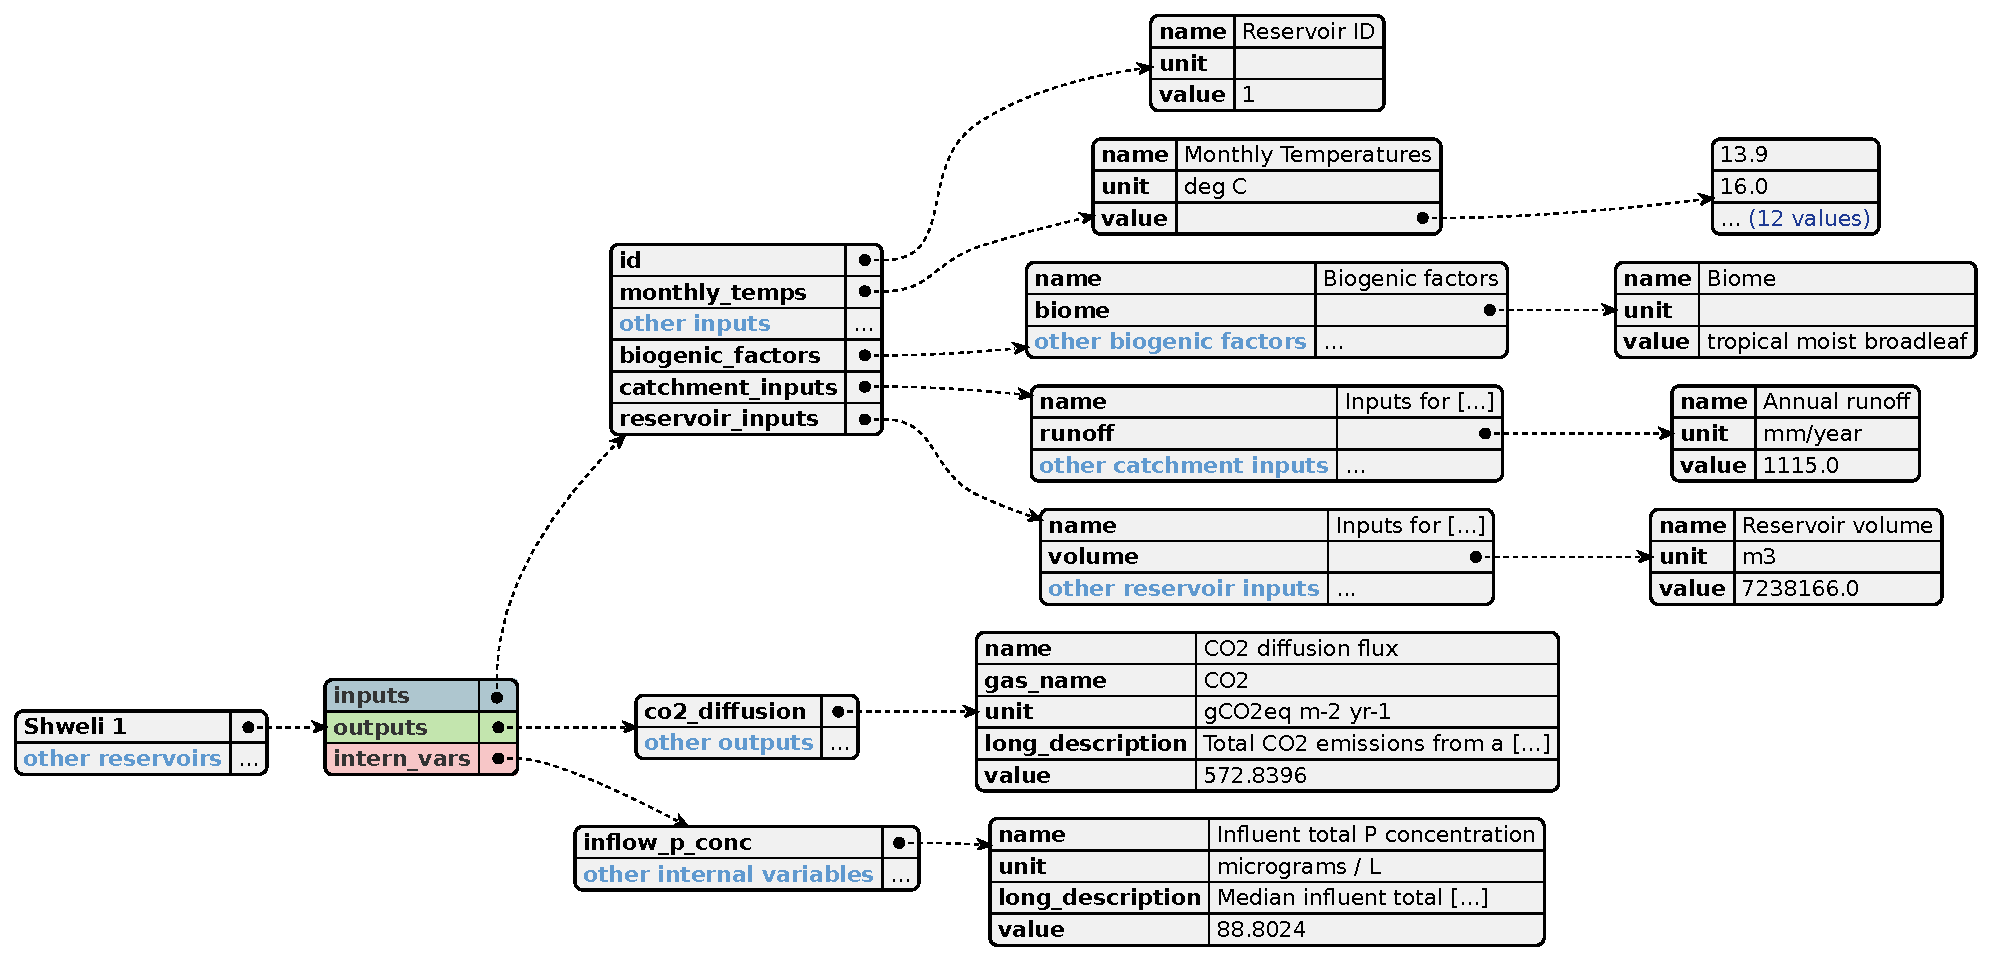
\includegraphics[width=0.9\textwidth]{figures/output_data_json.pdf}
    \caption{Structure of an example configurable output JSON file. The file is organized into three sections -- inputs, outputs, and internal variables -- highlighted in steel blue, olive green, and salmon, respectively. As the number of output entries can be arbitrarily large, selected values have been truncated for readability. Truncated content is indicated using light blue font colour followed by an ellipsis.}
    \label{fig:output_data_format}
\end{figure}

\subsection{Configuration options}
\label{subsec:config_options}

Configuration data -- including model parameters, options for the \vrbbrk{Presenter} class, and tabular inputs such as pre-impoundment emission factors or nutrient export coefficients -- is stored in INI and YAML files. 
These files provide semi-structured data representations that can be readily loaded into Python as dictionary objects.
The structure of these configuration files is illustrated in Figure~\ref{fig:config_uml} for presentation and model settings, Figure~\ref{fig:preimpoundment} for pre-impoundment emission factors, and Figure~\ref{fig:tp_tn_exports} for the parameterization of nutrient export models.

Configuration data is managed by the \vrbbrk{ConfigLoader} class, which registers configuration files and loads them lazily upon first access.
It also supports overriding default settings with user-defined configurations.
Instances of \vrbbrk{ConfigLoader} with registered configuration files are made globally accessible through the \vrbbrk{reemission.registry} module.

\subsection{Containerized execution using Docker}
\label{subsec:docker}

To ensure reproducibility and simplify the deployment of Re-Emission, we implemented a fully containerized workflow using Docker~\cite{merkel2014docker}, GitHub Actions, and the \acf{GHCR}, as illustrated in Figure~\ref{fig:docker_containerizing}.
This approach guarantees consistent runtime behaviour across computing environments and eliminates the need for complex setup procedures, thereby lowering the technical barrier to adoption.
Docker is an open-source platform that packages applications and their dependencies into standardized units called containers, which run in isolated environments.
Re-Emission, along with the Python interpreter, essential libraries, and other dependencies, is encapsulated in a Docker image.
The source code and Docker configuration files (e.g., \verb|compose.yaml|) are maintained in a GitHub repository, with \ac{CI} managed via GitHub Actions. Whenever changes are pushed to the \verb|release| branch, a Docker image is automatically built and published to the GitHub Container Registry.
This image can be retrieved using the standard \verb|docker pull| command, assuming Docker is installed on the user's machine.

The Re-Emission \ac{CLI} can be executed via \verb|docker compose run reemission| from a directory containing the appropriate \verb|compose.yaml| configuration file.
This file is required at runtime to map directories between the container and the host system, enabling access to input files and writing of output results.
To further streamline the Dockerized execution of Re-Emission, a companion repository is provided that defines the necessary folder structure, configuration files, and volume mappings for running the Re-Emission container~\cite{janus_geocaret_reemission}; see \emph{Software Availability}.

Currently, the shared Docker images for Re-Emission do not include a \LaTeX\ distribution, which is required for generating PDF reports via the \verb|pylatex| library.
This exclusion is deliberate, as bundling a full \LaTeX\ system -- such as TeXLive -- would significantly increase the image size, reducing portability and practicality for lightweight deployments.
Consequently, PDF report generation is not supported in the standard containerized version of Re-Emission.
However, equivalent HTML-based reports can be generated as described in Section\ref{subsec:input_output_formats}.
Users requiring PDF report generation within Docker must build a custom image by extending the official Re-Emission image with a \LaTeX\ installation.
This can be achieved by creating a new Dockerfile (see Listing~\ref{lst:docker_with_latex}) and building the image using the command \verb|docker build -t reemission-with-latex .| executed in the directory containing the Dockerfile.

\begin{figure}[ht]
    \centering
    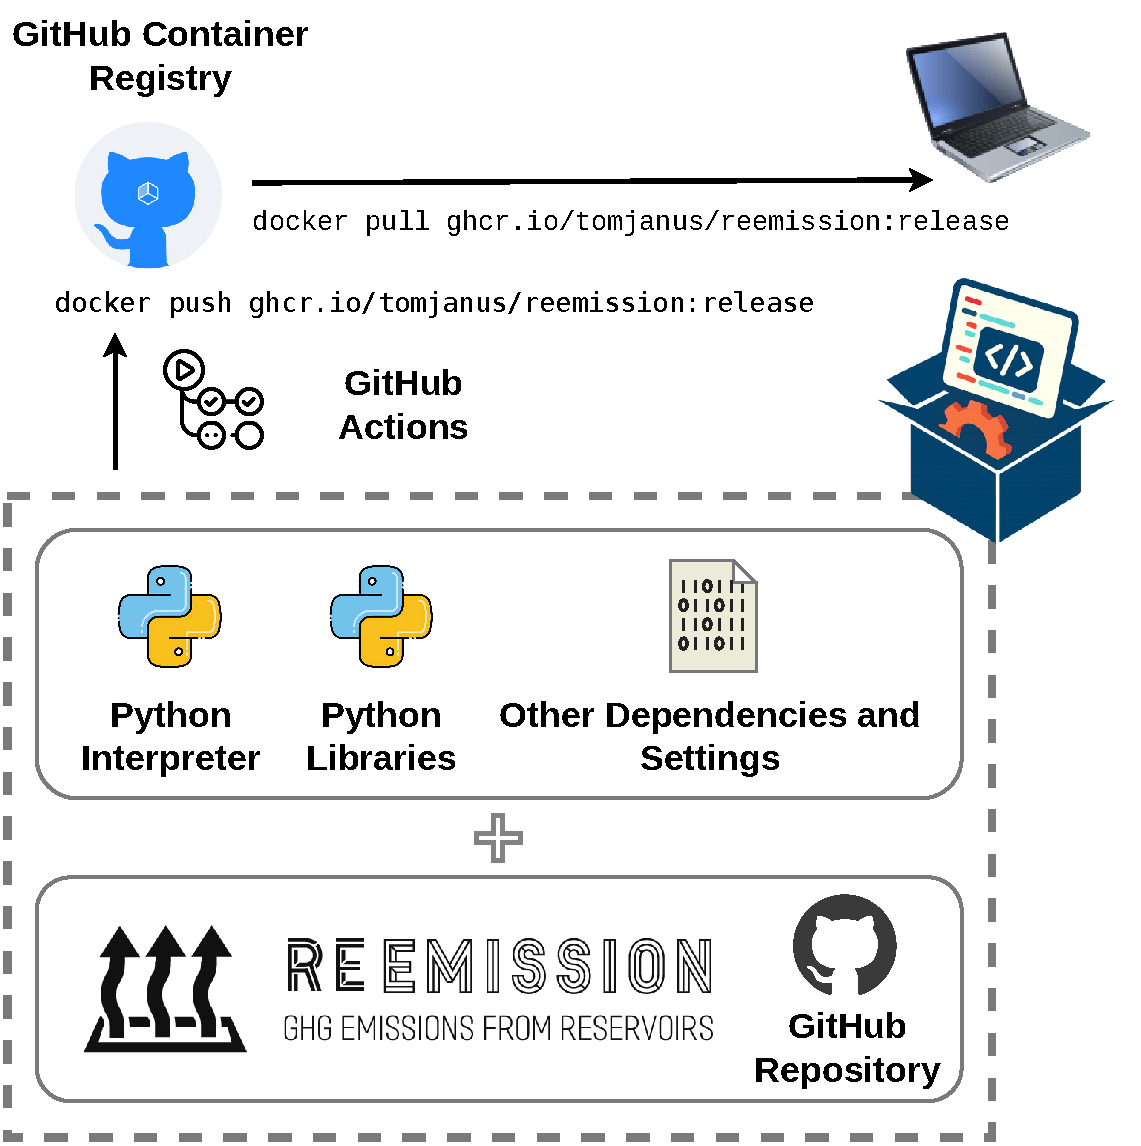
\includegraphics[width=0.55\textwidth]{figures/docker-explanation.drawio.pdf}
    \caption{{Containerized deployment of Re-Emission using Docker, GitHub Actions, and the GitHub Container Registry.}}
    \label{fig:docker_containerizing}
\end{figure}

\begin{minipage}{0.95\textwidth}
\begin{lstlisting}[language=Dockerfile, , label={lst:docker_with_latex}, caption={Dockerfile for extending the Re-Emission image with a full TeX Live installation to support PDF report generation via PyLaTeX.}]
# Dockerfile
FROM ghcr.io/tomjanus/reemission:release
# Install TeX Live
RUN apt-get update && \
    apt-get install -y texlive-full && \
    apt-get clean && \
    rm -rf /var/lib/apt/lists/*
\end{lstlisting}
\end{minipage}

\section{Integration with upstream reservoir and catchment processing}
\label{sec:integration}

The principal challenge in estimating emissions from multiple reservoirs using spatially explicit emission models such as G-res lies in the manual effort and time required to source and derive the necessary input data.
When input variables are not directly available, they must be extracted from geospatial datasets using various \ac{GIS} methods.
This typically involves delineating each reservoir and its corresponding catchment area, followed by processing diverse datasets such as \acp{DEM}, land cover maps, soil and biome classification layers, and various climate-related datasets.
These steps are often labour-intensive and time-consuming, particularly at larger spatial scales.

To streamline this process, we provide functionality for generating input JSON files for Re-Emission from the outputs of the open-source Geospatial CAtchment and REservoir analysis Tool (GeoCARET)~\cite{heettool}.
GeoCARET defines algorithms for a variety of statistical and geometric operations required to derive reservoir and catchment characteristics, and executes them on \ac{GEE}~\cite{Gorelick2017} via its Python API.
This setup enables automated data acquisition and preprocessing across multiple reservoir sites with minimal overhead, supplying the necessary inputs for the G-res model.
While still in its development stage, GeoCARET was successfully applied to generate the input data for the two case studies presented here and in the recent study on hydropower planning with emission models~\citep{janus2025planning}.

Integration between the tools is supported through a suite of \ac{CLI} functions, illustrated in Listing~\ref{lst:integration_cli}, that:
(i) merge multiple tabular files and populate missing variables (e.g., those not derivable from geospatial datasets and requiring manual input);
(ii) convert tabular data to JSON format; and
(iii) optionally merge individual reservoir and catchment shapefiles to support the mapping and visualization of emissions.
The integration workflow is further streamlined by running both tools within their respective Docker containers, coordinated through the Re-Emission--GeoCARET companion repository~\cite{janus_geocaret_reemission} introduced earlier (see \emph{Software Availability} for details).

\begin{minipage}{0.95\textwidth}
\begin{lstlisting}[language=bash, 
label={lst:integration_cli}, caption={Re-Emission CLI: Processing outputs from the GeoCARET reservoir and catchment processing tool.}]
# Step 1: Processing tabular GeoCARET outputs in multiple .csv files 
> reemission-geocaret process-tab-outputs \
    -i  geocaret_outputs.csv \
    -o  reemission_inputs.csv \
    -cv 'c_treatment_factor' 'primary (mechanical)' \
    -cv 'c_landuse_intensity' 'low intensity' \
    -cv 'type' 'potable'
# Step 2: Creating Re-Emission input JSON file from the tabular CSV data
> reemission-geocaret tab-to-json 
    -i reemisison_inptus.csv 
    -o reemission_inputs.json
# Step 3: Merging shape files (one per individual reservoir, catchment, dam, etc.) into combined shapes per geometry type
> reemission-geocaret join-shapes \
    -i  input_folder
    -o  output_folder
    -gp 'R_*.shp, C_*.shp, PS_*.shp'
    -f  'reservoirs.shp, catchments.shp, dams.shp'
\end{lstlisting}
\end{minipage}

%% Use \subsubsection, \paragraph, \subparagraph commands to 
%% start 3rd, 4th and 5th level sections.
%% Refer following link for more details.
%% https://en.wikibooks.org/wiki/LaTeX/Document_Structure#Sectioning_commands

%% Refer following link for more details.
%% https://en.wikibooks.org/wiki/LaTeX/Floats,_Figures_and_Captions
%% https://en.wikibooks.org/wiki/LaTeX/Importing_Graphics#Importing_external_graphics

\section{Emission model validation}
\label{sec:validation}

We conducted two validation experiments to evaluate the correctness of Re-Emission's implementation of the G-res model and to ensure that no computational or numerical inconsistencies were introduced through the integration of ancillary modules for data input, configuration management, and results presentation.

First, the G-res model was independently re-implemented in the R programming language following its original formulation by \citet{Prairie2021}.
Both implementations were used to compute key outputs, including gross and net areal CO$_2$ and CH$_4$ emissions across all modelled pathways, as well as intermediate diagnostic variables involved in the emission calculations.
By systematically cross-comparing outputs and reviewing the source code of both implementations, we minimized the likelihood of algorithmic or implementation-level discrepancies.
To assess model fidelity across a wide range of input conditions, we generated a synthetic validation dataset by randomly perturbing categorical variables in the input data representing real reservoirs.
This approach allowed exploration of parameter combinations not represented in empirical case studies.
The resulting dataset comprised 246 reservoirs generated from modified instances of real systems located in Myanmar and the United Kingdom, spanning diverse land-cover types, biomes, climatic regimes, soil classes, land-use intensities, and catchment-scale treatment factors.
Comparison of outputs between Re-Emission and the R-based reference implementation is presented in Figures~\ref{fig:validation_plot_gross_emissions} and~\ref{fig:validation_plot_net_emissions}.
The results demonstrate near-perfect agreement across gross areal emissions by pathway (Figure~\ref{fig:validation_plot_gross_emissions}), pre-impoundment emissions (Figure~\figref[a]{fig:validation_plot_net_emissions}), and net anthropogenic emissions (Figure~\figref[b]{fig:validation_plot_net_emissions}), with coefficients of determination ($R^2$) equal to 1.000 in all cases.

Additionally, we selected four real reservoirs from Myanmar and the United Kingdom and estimated their emissions using both Re-Emission and the G-res Tool v3.31.
The corresponding comparisons are presented in Supplementary Figures~1 -- 3.
The results show near-perfect correspondence between the two implementations for both gases (CO$_2$ and CH$_4$) and across all modelled pathways, encompassing both average annual gross and net emissions as well as emission profiles over time.
These findings confirm that Re-Emission faithfully reproduces the behaviour of the published G-res model~\cite{Prairie2021} and its web-based public implementation (G-res Tool v3.31), providing reliable emission estimates across a wide range of environmental and geographical contexts.

\begin{figure}[ht]
    \centering
    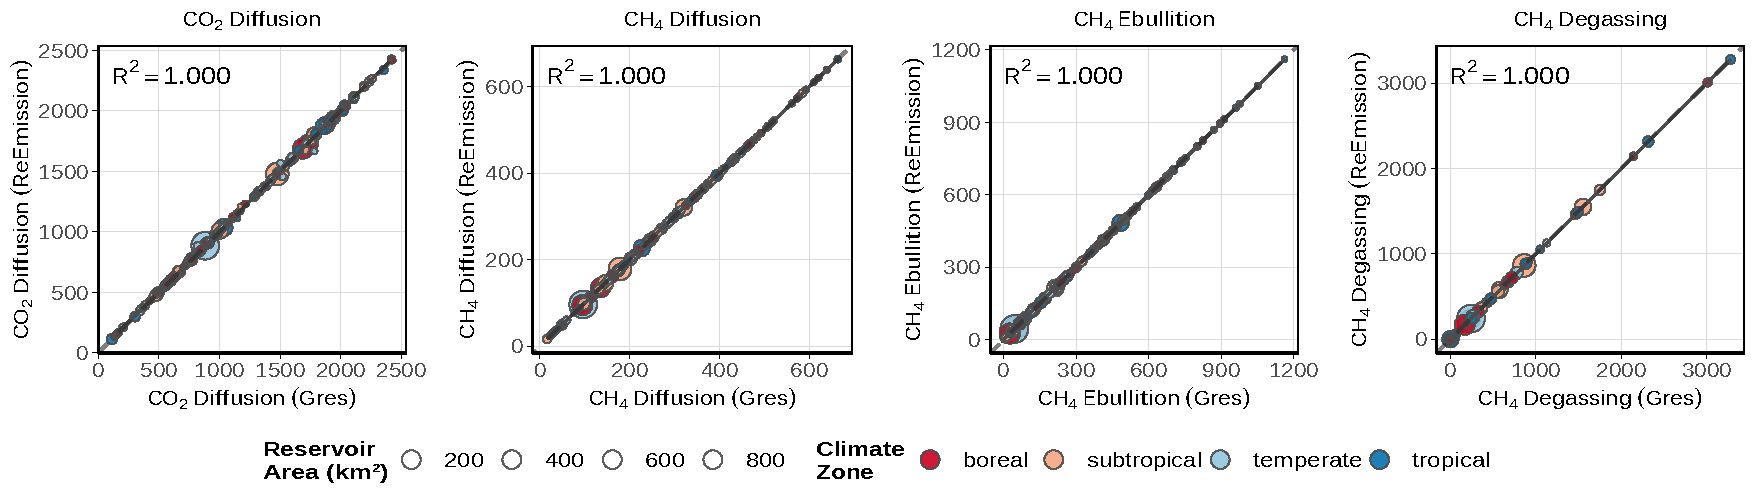
\includegraphics[width=1.0\textwidth]{figures/comparison_plot.pdf}
    \caption{{Comparison of gross areal emissions (in gCO$_{2e}$ m$^{-2}$ yr$^{-1}$) via four emission pathways -- CO$_2$ diffusion, CH$_4$ diffusion, CH$_4$ ebullition, and CH$_4$ degassing (from left to right) -- predicted using Re-Emission (y-axis) and the R-based G-res implementation (x-axis).}}
    \label{fig:validation_plot_gross_emissions}
\end{figure}

\begin{figure}[ht]
    \centering
    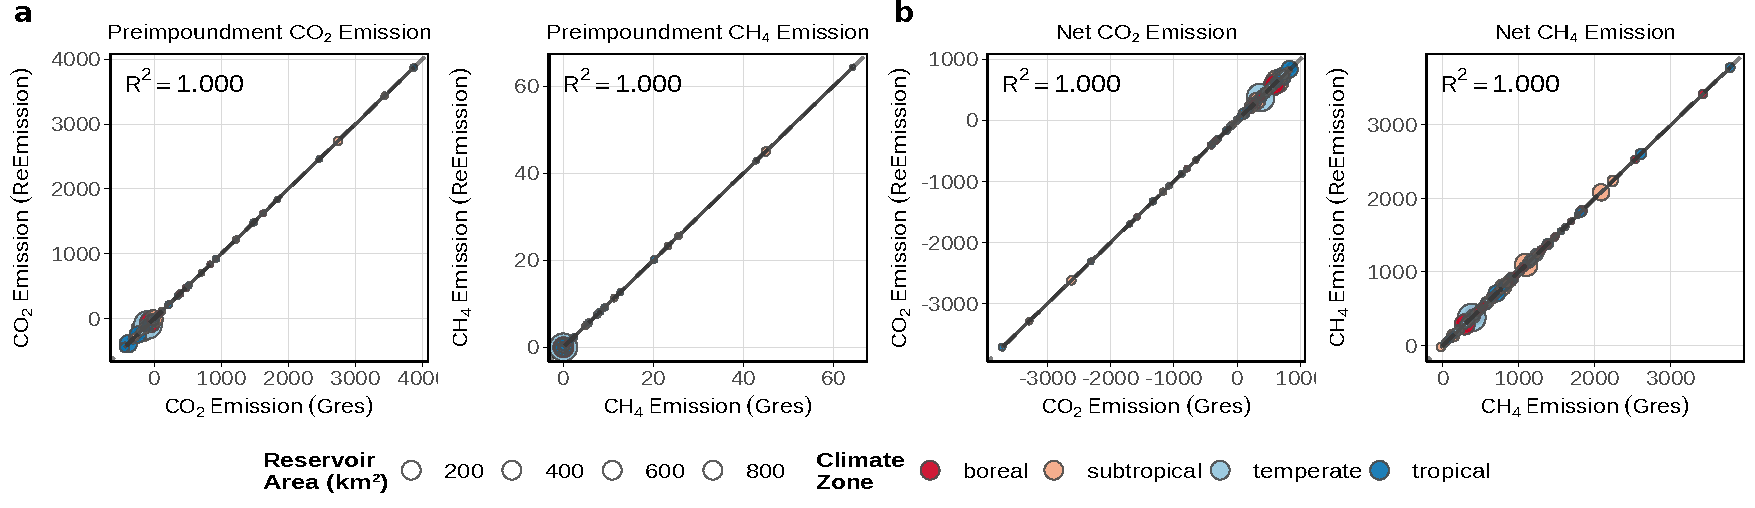
\includegraphics[width=1.0\textwidth]{figures/comparison_plot_net_emissions.pdf}
    \caption{{Comparison of (a) areal pre-impoundment CO$_2$ and CH$_4$ emissions and (b) areal net anthropogenic CO$_2$ and CH$_4$ emissions (both in gCO$_{2e}$ m$^{-2}$ yr$^{-1}$) predicted using Re-Emission (y-axis) and the R-based G-res implementation (x-axis).}}
    
    \label{fig:validation_plot_net_emissions}
\end{figure}

\section{Case Studies}
\label{sec:case_studies}

We present two case studies to demonstrate key functionalities of Re-Emission for estimating \ac{GHG} emissions from reservoirs: (i) the estimation of total life-cycle emissions and emission profiles at scale, and (ii) the assessment of emissions under parametric uncertainty.
The first case study illustrates how Re-Emission facilitates emission assessments across multiple reservoirs, for example at regional or national scales. The second case study demonstrates the integration of Re-Emission with the Python-based sensitivity analysis library SALib~\cite{Iwanaga_Toward_SALib_2_0_2022}, enabling exploration of global sensitivity and uncertainty in emission predictions due to uncertain model parameters.
This functionality has both practical and scientific significance: it supports robust decision-making and contributes to methodological advancements in reservoir emission modelling.
To the best of our knowledge, the influence of uncertainties -- particularly input uncertainties -- on emission estimates has received limited attention in the existing literature.
Re-Emission helps address this gap by enabling uncertainty and sensitivity analysis of emission models with SALib.
The source code for reproducing the results of both case studies is available on GitHub and archived on Zenodo -- see \emph{Data availability}.

\subsection{Emission trajectories from existing and planned assets in Myanmar}
\label{subsec:myanmar}

In this case study, we assess the temporal evolution of biogenic \ac{GHG} emissions from more than 200 existing and planned reservoirs in Myanmar. 
Myanmar possesses substantial untapped hydropower potential, estimated at over 100~GW of identified capacity~\citep{EA_Myanmar} and is looking to triple its hydropower capacity by 2030~\citep{Aung2020}; however greenhouse gas implications of such large-scale development remain poorly understood. 
Moreover, emissions from existing irrigation reservoirs -- of which there are many -- have received limited attention despite their potentially significant atmospheric impact.

Using the Re-Emission framework, we estimated biogenic emissions from all identified \acf{IRR}, \acf{MP}, and \acf{HP} reservoirs in Myanmar known to us.
For each reservoir, emission profiles -- representing the temporal evolution of biogenic emissions following impoundment -- were generated and subsequently aggregated to derive national-scale reservoir emission trajectories.
This was achieved using Re-Emission's emission profile generation and aggregation module, which allows simulation and temporal aggregation of emissions from multiple reservoirs.
Additionally, we used Re-Emission as a Python library to generate aggregated emission trajectory ensembles under uncertain impoundment dates for existing and planned reservoirs, quantifying the range of plausible \ac{GHG} emission trajectories over a planning time-horizon.
Further methodological details are provided in the Materials and Methods section.

The ensemble results, illustrated in Figure~\ref{fig:mya_emission_profile}, reveal distinct temporal patterns across asset classes. 
Emissions from irrigation reservoirs appear to have peaked around 2005 and have declined steadily since, suggesting a maturing phase of irrigation infrastructure development. 
In contrast, emissions associated with planned \ac{HP} and \ac{MP} projects exhibit large uncertainty envelopes, reflecting variability in future commissioning timelines. 
These projects are projected to drive a pronounced rise in national biogenic emissions, with peak values likely between 2030 and 2050. 
Although emissions are expected to decline sharply following the peak, they remain above current levels through at least 2060. 

Overall, the analysis indicates that future reservoir development could substantially alter Myanmar's national emission profile. 
The insights illustrated in Figure~\ref{fig:mya_emission_profile} can inform national \ac{GHG} mitigation strategies and guide infrastructure planning.
Re-Emission's capability to dynamically alter model parameters also allows straightforward extension to other uncertainty types -- such as model parameter uncertainty -- as shown in the next case study.

\begin{figure}[ht]
    \centering
    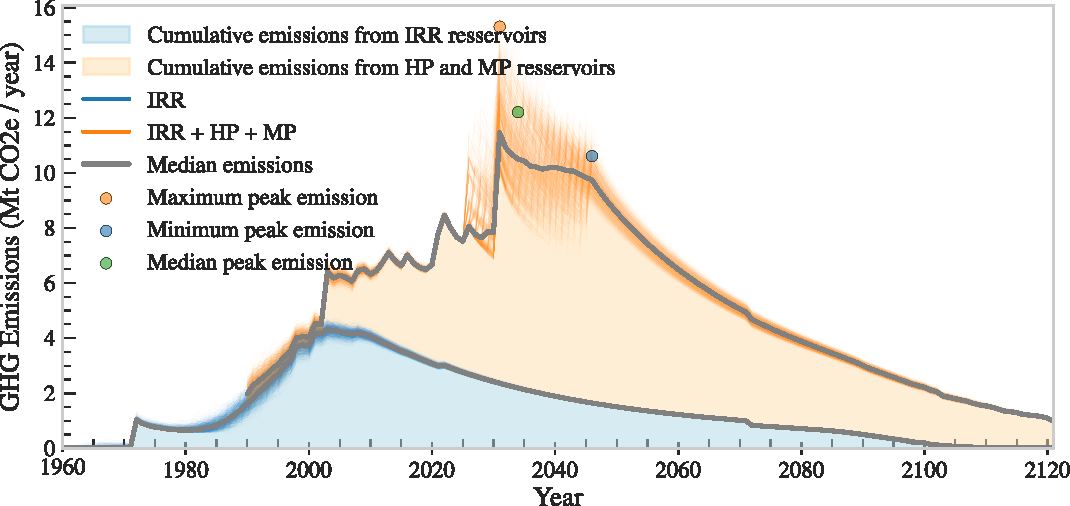
\includegraphics[width=0.8\textwidth]{figures/emission_profile.pdf}
    \caption{{Projected temporal evolution of emissions from existing and planned irrigation (IRR), multipurpose (MP), and hydroelectric (HP) reservoirs in Myanmar. In the absence of impoundment date information for some hydroelectric and multipurpose reservoirs, a 20-year planning horizon is assumed, by which all reservoirs included in current hydropower expansion plans are expected to be completed.}}
    \label{fig:mya_emission_profile}
\end{figure}

\subsection{Uncertainty analysis of reservoir emissions in Scotland and Wales}
\label{subsec:scotland_wales}

While it is widely acknowledged that emission model predictions are subject to considerable uncertainty, the magnitude and sources of these uncertainties remain poorly characterized. 
Reservoir emissions result from complex biogeochemical processes that are difficult to observe, model, and generalize due to their inherent spatio-temporal variability and often poorly understood dynamics.
Consequently, models developed from limited observational data may exhibit substantial epistemic and parametric uncertainties.
In addition, emission models typically rely on a large number of input variables -- many derived from geospatial datasets -- which themselves carry varying degrees of uncertainty.
These factors lead to compounded uncertainty in model outputs, with important implications for the reliability of emission estimates as a basis for decision-making and policy design.
Enabling uncertainty analysis and probabilistic emission estimation under parameter and input uncertainty is therefore of practical value to both researchers and practitioners.

To demonstrate these capabilities in Re-Emission, we conducted an analysis of parametric uncertainty in the G-res diffusive CO$_2$ and CH$_4$ emission models and evaluated their effect on total net anthropogenic emission estimates. 
The governing equations for diffusive CO$_2$ and CH$_4$ fluxes are provided in Equations 7 and 3 of \cite{Prairie2021}, respectively.
As the objective of this section is to illustrate the application of the software rather than to perform a full quantitative sensitivity analysis, the analysis was restricted to diffusive emissions only.
This analysis was applied to 20 reservoirs located in Wales and Scotland. 
%The results are summarized in Figure~\ref{fig:uncertainty_analysis}. 
The results show that in this case, uncertainty in total net emission estimates is largely driven by the CO$_2$ diffusion process (Figure~\figref[b]{fig:uncertainty_analysis}), particularly the ``$\textrm{k}_1\,\textrm{diff}\,\textrm{co2}$'' coefficient. Coefficients ``$\textrm{k}_6\,\textrm{diff}\,\textrm{co2}$'' and ``$\textrm{k}_1\,\textrm{diff}\,\textrm{ch4}$'' also contribute to output variability, but their influence varies across reservoirs. This suggests that their importance is context-dependent, likely influenced by site-specific conditions or the relative contribution of individual emission pathways. 
Total net emission estimates for all 20 reservoirs, along with 95\% prediction intervals, are shown in Figure~\figref[c]{fig:uncertainty_analysis}.
The variability in prediction intervals across reservoirs is evident and again largely attributable to CO$_2$ diffusion uncertainty.
Figure~\figref[d]{fig:uncertainty_analysis} presents the probability density function of total net emissions for the Baddingsgill reservoir, illustrating the spread of values and indicating the mean, median, nominal estimate, and 5$^\textrm{th}$ and 95$^\textrm{th}$ percentiles.

Although this case study is intended for demonstration purposes, the approach can be readily extended to include additional parametric and input uncertainties -- both of which are supported by Re-Emission.
Due to the computational demands of Sobol analysis, however, expanding the number of uncertain parameters may require access to higher performance computing resources.
Assessing reservoir emissions under uncertainty remains an open research area, and Re-Emission provides a flexible and extensible platform for advancing such analyses.

\begin{figure}[!h]
    \centering
    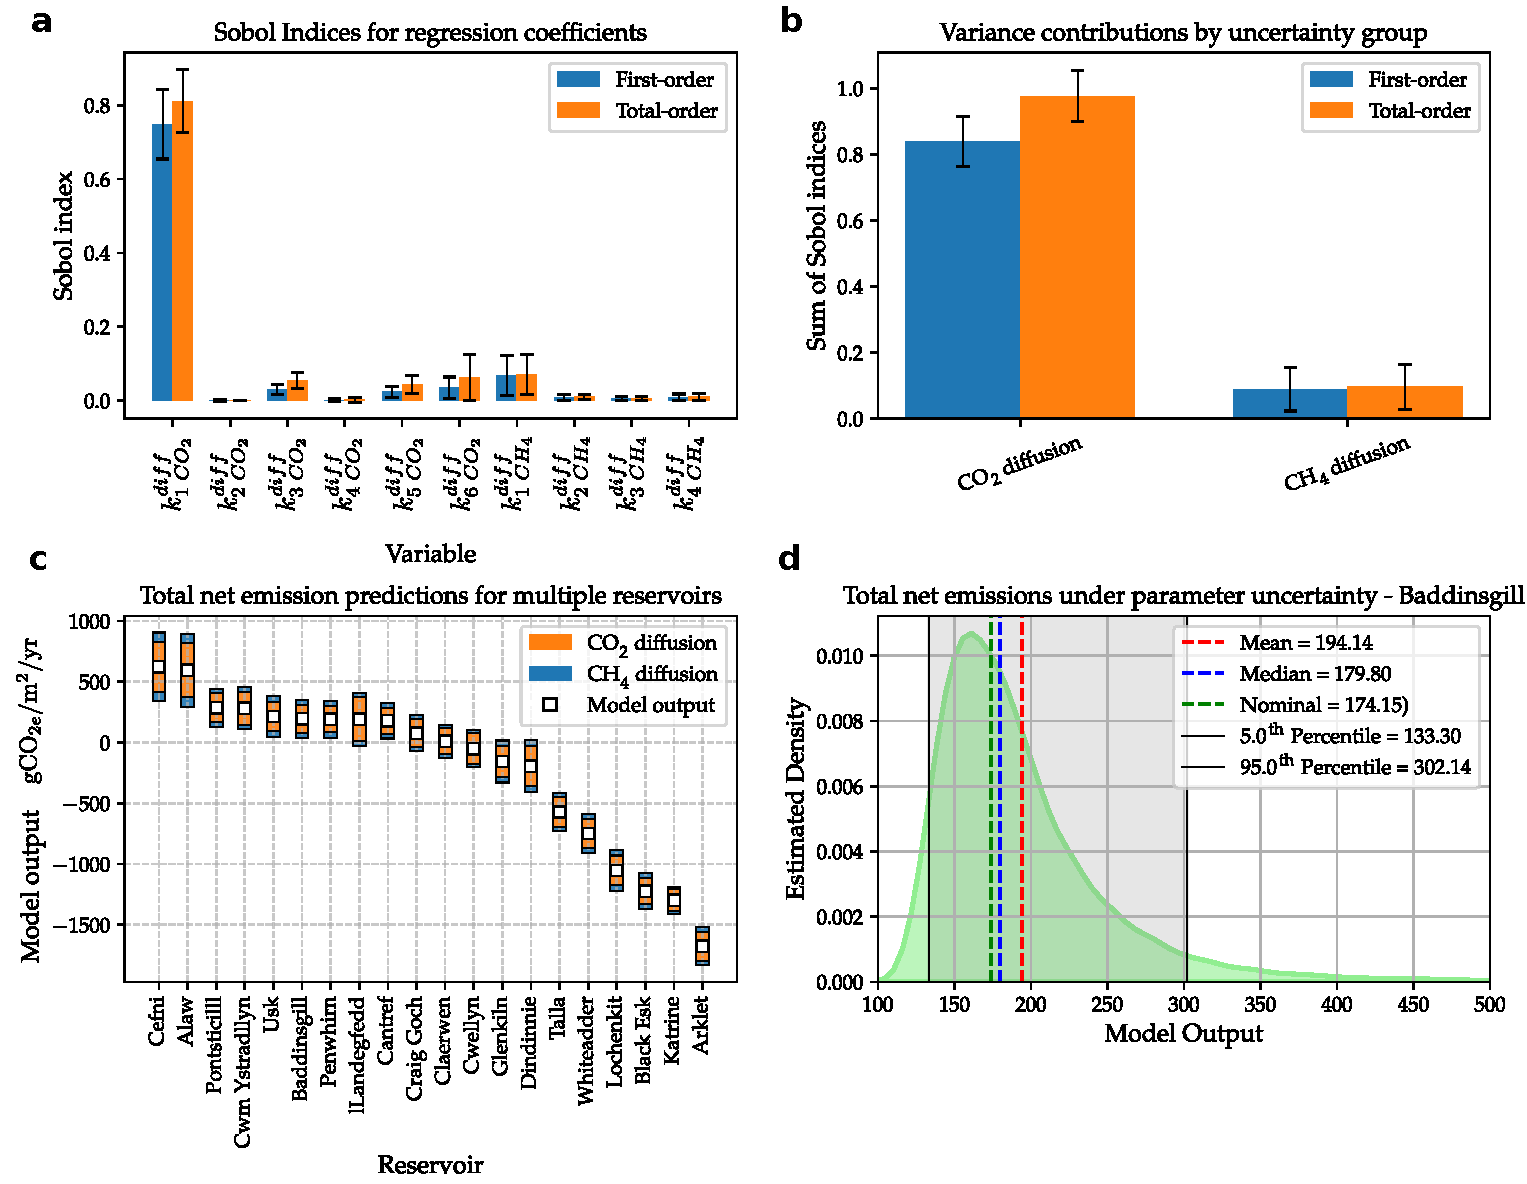
\includegraphics[width=1.0\textwidth]{figures/reemission_sobol_paper.pdf}
    \caption{
Quantification of parametric uncertainty in total net emissions from CO$_2$ and CH$_4$ diffusion processes for 20 reservoirs in Wales and Scotland. 
\textbf{(a)} First-order and total-order Sobol indices for the CO$_2$ and CH$_4$ diffusion regression coefficients, with error bars indicating variability across reservoirs. 
\textbf{(b)} Aggregated Sobol indices (first- and total-order) grouped by sources of uncertainty. 
\textbf{(c)} Total net emission estimates for the 20 reservoirs, with error bars indicating 95\% prediction intervals; the contribution of each uncertainty group is colour-coded. 
\textbf{(d)} Probability density function of total net emissions for a selected reservoir, with mean, median, nominal values, and the 5$^\textrm{th}$ and 95$^\textrm{th}$ percentiles indicated.
}
    \label{fig:uncertainty_analysis}
\end{figure}


% ----- for information only ------
%The mineral/organic soil partitioning is derived from the ‘soil grids’ global layers, from which the soil C content is calculated as the mean C content of the inundated reservoir area and provided in the variable \verb|r_msocs_kgperm2|. It is required for distinguishing mineral from organic soils in the impounded/inundated reservoir area in order to apply correct \ac{IPCC} default tier1 ghg emission factors by climatezone and landcover type to estimate pre-impoundment GHG fluxes. 
%(seek definition) The organic soils are broadly peats that are positioned deeper than 40cm in the soil column and are thus somewhat restricted to specific areas (boreal, temperate uplands (Scotland), tropical uplands (andes) and basins (Congo) and SW Asia, such as Indonesia , with lots of palm on peat).
%(Chris) The general and \ac{IPCC} definition of organic soils (see image at end of this mail- I don’t find this free of ambiguity but anyway) is that they contain $>$12\% organic carbon by weight in the 0-30cm soil horizon.
%If 40 kg OC m-2 is expressed as a \% of soil volume (GRES text), with 1g OC incorrectly taken as = 1cm3 and 1cm3 soil = 1 g soil, for the 0-30cm strata, we get total mass or vol of soil in 0-30cm for 1m2 = 300kg or 300dm3 or 0.3 m3
%40 / 300 = 0.13 = 13.3\%  SOC – this is close to the threshold of 12\%   (although 36 kg m-2 would yield exactly 12\% by this approach).
%This is incorrect and indeed there are no global incidences of  $>$c.25 kg OC m-2 for the 0-30cm soil horizon. Aside from my speculation I cannot see how gres may have estimated the \% OC from the soil OC stock data (t/ha for 0-30cm), or how to consolidate their approach with the \ac{IPCC} org soil definition. 
%What we need to try to do to get correct soil classification among Min and Org soils:    derive \% SOC for 0-30cm.
% ----- for information only ------

\section{Materials and Methods}
\label{sec:materials_and_methods}

\subsection{Calculation of emission trajectories}
\label{subsec:myanmar_case_study_methods}

Information on existing and planned reservoirs -- including their locations, physical characteristics, and, where available, impoundment years -- was compiled from a range of open and country-specific databases and reports~\citep{ifc_dam_db, EA_Myanmar, Emmerton2015, opendevelopmentmya2018, PowerSector_Myanmar, sea2018}.
Emissions from individual reservoirs were explicitly estimated using Re-Emission, with input data derived from global open datasets processed via GeoCARET, as described in \citet{janus2025planning}.

Missing impoundment years were reconstructed using a hybrid stochastic procedure.
For irrigation reservoirs, known impoundment years were used to estimate the probability density of historical development via kernel density estimation (\acs{KDE}).
Synthetic impoundment years were then sampled from the resulting density function to impute missing values, thereby preserving temporal patterns in irrigation reservoir infrastructure expansion.
Empirical adjustments were applied to align with observed construction activity (e.g., approximately 12~dams per year during 1988--1995) and to maintain continuity across under-reported periods (1979--1988 and 1997--2010).
For planned \ac{HP} and \ac{MP} dam projects, reservoir impoundment years were sampled from a uniform distribution spanning 2025 -- 2045, consistent with Myanmar’s hydropower expansion targets~\citep{Aung2020}.

Uncertainty in impoundment dates of under-reported reservoirs was propagated through Monte Carlo sampling, generating 1,000 realisations covering the 1965 -- 2045 period.
Each realisation represented a distinct combination of reservoir impoundment sequences, for which annual CO\textsubscript{2} and CH\textsubscript{4} flux profiles were simulated using Re-Emission.
Scenario results were aggregated across reservoirs to produce national time series of net biogenic reservoir emissions.
The ensemble was summarised using the median and percentile bounds of total annual emissions, disaggregated by reservoir type.
Results are reported for two planning horizons: 2035 and 2040, representing near- and mid-term emission trajectories under infrastructural uncertainty.

\subsection{Parametric uncertainty analysis}

Parametric uncertainty was evaluated using a global variance-based approach implemented through the Sobol' method~\citep{Sobol2001}. 
This method decomposes the total output variance into contributions from individual uncertain parameters and their higher-order interactions.
The first-order ($S_1$) and total-effect ($S_T$) Sobol indices were calculated to quantify, respectively, the direct and overall influence of each parameter on the variability of net diffusive CO$_2$ and CH$_4$ emissions.

Re-Emission facilitates the quantification of parametric and input uncertainty through an interface to the Python-based sensitivity analysis library {SALib}~\citep{Iwanaga_Toward_SALib_2_0_2022}. 
This integration enables global sensitivity analysis using the Sobol' method~\citep{Sobol2001, Saltelli2002} and supports Monte Carlo simulations under user-defined uncertainty descriptions. 
The interface leverages Re-Emission's modular configuration system, allowing changes of model parameters such as regression coefficients, pre-impoundment emission factors, or nutrient export rates, to be made dynamically during and in between model runs. 
Both parametric and input uncertainties can be propagated, and multiple probability distributions---including continuous, discrete, and categorical forms---are supported.

Uncertain parameters were defined in a dedicated YAML specification file that included access statistical descriptions of each uncertain variable. 
Here, normal distributions were assumed for all regression coefficients, with standard deviations adopted from \citet{Prairie2017b_old} -- the technical documentation (v2.21) of the G-res Tool. 
Because this documentation predates the current G-res implementation (v3.31) and reports slightly different parameter values, the analysis presented here is illustrative, demonstrating the functionality of the {Re-Emission}-{SALib} framework rather than providing definitive estimates of parametric uncertainty in G-res diffusive emissions.

The inputs to Monte-Carlo uncertainty propagation were generated using quasi-random Sobol sampling~\citep{Saltelli2002}, with sample sizes ranging from 2{,}048 to 8{,}192 realisations per reservoir. 
Each realisation represented a unique parameter combination for which {Re-Emission} computed net annual mean CO$_2$ and CH$_4$ emission fluxes. 
The uncertainty propagation problem was constructed using the \texttt{ReEmissionSALib} interface, which automates parameter initialisation, problem definition, and execution of the complete Sobol analysis workflow.

For each reservoir, ensemble outputs were analysed to derive Sobol indices and probability distributions of net emissions. 
Sensitivity indices were computed for each parameter and aggregated by emission pathway to identify dominant sources (emission processes) contributing to emission prediction uncertainty at both the reservoir and aggregate levels. 
Kernel density estimation was applied to ensemble results to visualise the probability distributions of predicted diffusive emissions under parametric uncertainty.


\section{Discussion}
\label{sec:discussion}

This study addresses a gap in the current technological landscape that has limited the ability of scientists and practitioners to estimate reservoir \ac{GHG} emissions at scale, explore alternative emission model formulations, and incorporate such models into broader system-level analyses beyond single-reservoir applications.
To address these challenges, we developed an open-source software tool that implements and extends the G-res framework, enabling large-scale, automated assessments of reservoir emissions through a seamless interface with GeoCARET~\cite{heettool} - an automated reservoir and catchment processing tool.
The software’s capabilities were demonstrated in two case studies, highlighting its scalability, configurability, and support for advanced analyses, including uncertainty quantification and probabilistic modelling.
While the tool represents a substantial advancement in the field of modelling reservoir emissions, certain limitations remain, motivating future development.
These limitations, along with the tool's benefits and proposed directions for further work, are discussed in the following sections.

\subsection{Limitations}
\label{subsec:limitations}

Despite its several advancements over existing software, Re-Emission currently exhibits notable limitations that warrant further development.
Although the tool offers some flexibility for incorporating new models, it is presently centred on implementing and extending the G-res model, with the primary goal of making this implementation both adaptable for customized analyses and practical through configuration and visualization options.
However, it cannot yet be considered a general-purpose framework capable of accommodating a broad spectrum of modelling paradigms (e.g., process-based approaches or dynamic models).
Second, because Re-Emission integrates the G-res model along with several extensions, it inherits the limitations, biases, and uncertainties associated with these formulations.
Third, the current implementation does not support the simulation of emissions from cascading reservoir systems -- that is, series of reservoirs in which the outflow of one forms the inflow of another.
This limitation arises primarily from constraints within the G-res model itself, but also from the present design of the Re-Emission framework.
Consequently, it is not particularly suited for basins dominated by cascading reservoir systems, where reservoir interactions may play a key role in emission dynamics.
Finally, Re-Emission is not yet equipped to integrate emission models for other aquatic systems, such as rivers and streams \citep{Rocher-Ros2023}, lakes \citep{Zhuang2023}, or wetlands \citep{Hu2024}.
Although modelling frameworks for these systems are still under development, future applications will likely require tools that enable multi-system integration.
Progressing towards integrated assessments of greenhouse gas and nutrient budgets at the catchment scale will be essential for achieving spatially resolved and transparent representations of aquatic contributions to the global carbon cycle.

\subsection{Benefits}
\label{subsec:benefits}

The \emph{Re-Emission} package advances the state of the art in modelling reservoir \ac{GHG} emissions by providing a programmatic solution that supports batch processing and facilitates the scaling of emission assessments to multiple reservoirs.
In addition, it systematizes the modelling workflow for G-res and other prospective spatially explicit models that adopt similar conceptual frameworks. 
Its modular architecture and open-source nature allow users to extend the framework by incorporating new sub-models or applying custom parameterization, such as region-specific calibrations or updates based on new empirical data.
The importance of such model refinements and recalibrations has recently been emphasized by \citet{Pilla2025}.
Developed in Python -- one of the most widely used programming languages in scientific and engineering domains -- the tool can be seamlessly integrated into broader modelling pipelines.
This enables a wide range of applications, including the evaluation of emissions under parametric or input uncertainty, as well as integration with complementary tools such as GeoCARET for catchment and reservoir delineation, as demonstrated in this manuscript.
Finally, \emph{Re-Emission} provides a free and open-source alternative to existing solutions, offering cost-free emission analysis for both academic and commercial users.
Its transparent, modular, and automated design further promotes reproducibility and traceability in both research and applied contexts.

% ----- do not use this text ------
%designed to predict gross reservoir emissions via multiple emission pathways and quantify the share of net anthropogenic emissions
% and their underlying software is still limited.
%Overall, while the science of reservoir GHGs has advanced rapidly (from isolated measurements to global models), uncertainties are still large. Key research needs include more field data from underrepresented regions and reservoir types, better monitoring of all pathways (CH4, CO2, N2O), and refinement of predictive models (e.g. incorporating remote sensing of drawdown). In parallel, practitioners benefit from emerging tools: the G-res calculator and IPCC guidelines are widely used today, and new frameworks (e.g. automated geospatial models) are being developed to integrate GHG considerations into dam planning and policy.
%current ch4 measurements from Flooded Land are not sufficiently comprehensive to support the development of accurate default emission
%factors (especially for bubbles emissions and degassing emissions). 
%there is a lack of comprehensive data on the emission rates, dominant pathways and influence of various factors on emissions in reservoirs of different sizes, morphologies and locations. 
%The work is limited by the availability of data that cover a wide range of conditions in reservoirs  and identification of processes
%The significant share of reservoir emissions in global emissions combined with a growing reservoir storage globally (27.82$\pm$0.08~km$^3$/yr observed between 1999 and 2018~\cite{Li2023}) prompts for ...
% ----- do not use this text ------

\subsection{Future Work}
\label{subsec:future_work}

To address current limitations, future development of the Re-Emission will focus on enhancing modularity, interoperability, and flexibility to support next-generation assessments of reservoir \ac{GHG} emissions.
Although the current architecture is primarily centred on implementing the G-res model, we envision a transition to a network-based design that represents interconnected reservoirs and river reaches.
This structure would provide a more versatile foundation for modelling emissions from hydrologically connected water bodies and would overcome current limitations, such as the inability to represent cascading reservoir systems.

In this envisioned framework, carbon and nutrient mass balances would need to be explicitly solved, acknowledging their inherent biogeochemical interlinkages and coupled and differential cycling with respect to \ac{GHG} emissions and ecosystem impacts across the land--ocean continuum (e.g.,~\cite{Nixon2003,Maranger2018,Maavara2020}). 
Mass balance approaches that incorporate such stoichiometric dependencies have already shown promise in reducing uncertainties in reservoir \ac{GHG} emission estimates and are particularly well suited for extension to cascading systems (e.g.,~\cite{Delwiche2022}). 
Their broader application -- especially in the context of cascading reservoir networks -- is however dependent on the availability of higher-resolution spatio-temporal data and improved process-level understanding (e.g.,~\cite{grasset2021empirical}). 
Integrating one-dimensional hydrodynamic and water resources models (e.g.,~\cite{Almeida2022_temperatures}) with downstream thermal propagation simulations (e.g.,~\cite{Long2019_Jinsha,He2025a}) and coupling them with robust estimations of landscape and reservoir macronutrient exports (e.g.,~\cite{He2025b}) presents both opportunities and challenges for advancing the field, particularly towards representing time-varying, non-steady-state conditions driven by climate and land-use changes, as well as reservoir operational dynamics (e.g.,~\cite{Harrison2017}).

Further work should also focus on separating the core framework -- comprising foundational classes and metaclasses -- from specific model implementations to establish Re-Emission as a fully generic emission-modelling platform.
We envisage an architecture in which objects inheriting from shared parent classes (representing generic models and submodels) can be programmatically combined into interconnected composite models.
For example, the phosphorus input to the G-res model could be defined either as a fixed quantity or derived dynamically from a phosphorus-export submodel.
Such modular design would enable submodels to be interchanged with fixed inputs, allowing complex coupled models to be executed as seamlessly as single-model configurations.
This framework would simplify model construction through a high-level programming interface and make visualization and configuration components model-aware -- automatically adjusting required inputs, parameters, and display options based on the assembled model.
To further improve usability and automation, tighter integration with upstream geospatial processing tools such as GeoCARET should be pursued, enabling the automatic sourcing and pre-processing of reservoir and catchment input data.

Beyond architectural enhancements, future work must also address underrepresented emission pathways and processes.
Recent empirical studies have underscored the importance of previously unmodelled or not extensively modelled sources, such as e.g. via submerged macrophytes ~\citep{Hilt2022, Suraj2023} or downstream CH$_4$ degassing~\citep{Abbasi2020, Zhou2024} -- with the latter accounting in some cases for up to 90\% of total reservoir-related emissions~\citep{Deshmukh}.
Accounting for these pathways will likely require coupling with complementary models or developing new modules that incorporate dynamic environmental conditions, including water level fluctuations and wetting-drying cycles in littoral zones~\cite{Calamita2021, Ion2021} -- necessitating a re-evaluation of existing modelling architectures.
This would also help addressing limitations of the current G-res implementation, which relies on static regressions and inherits biases stemming from site selection and measurement techniques, by incorporating more process-based representations of emission drivers.
Although there is currently no direct replacement for the G-res framework and Re-Emission does not aim to substitute it, this work intends to enable community-driven improvements, extensions, and incorporation of new emission pathways, which will hopefully help advance the state of the art in reservoir emission modelling.

Finally, although \acf{N2O} is a highly potent climate forcer, it remains the least studied of the three major \acp{GHG} in aquatic systems and is not yet routinely included in reservoir emission models.
However, global estimates suggest that lakes and reservoirs emit substantial amounts of N$_2$O~\cite{Li2024}, and recent studies indicate that under certain conditions -- particularly in nutrient-rich or thermally stratified systems -- N$_2$O emissions may rival or even exceed those of CH$_4$~\cite{Chen2025}.
These findings underscore the urgent need for expanded empirical observations and for the systematic integration of \ac{N2O} into reservoir modelling frameworks to more accurately represent the cumulative climatic impact of inland waters.

% ----- do not use this text ------
%A further area for exploration is the refinement of parameterizations related to nitrogen and phosphorus exports and pre-impoundment emissions, particularly for less-studied land-cover types such as wetlands or organic soils. For instance, land uses on peatlands or high-organic-content soils may exhibit distinct biogeochemical behaviour that is not currently captured in most empirical models.
%($\sim$65 Gg N$_2$O N yr$^{-1}$ in the 2010s), yet its inclusion in models remains rare. Recent studies suggest that N$_2$O emissions may rival or exceed CH$_4$ in specific contexts~\cite{Chen2025}, particularly in nutrient-rich or thermally stratified systems. These findings highlight the urgent need for additional empirical data and model integration to better represent N$_2$O dynamics within emission assessment tools.
%Collectively, these future directions will advance the \emph{Re-Emission} framework toward a comprehensive, extensible platform capable of supporting robust and policy-relevant emission modeling across scales and regions.
%To enhance end‐to‐end automation, we will improve interoperability with upstream geospatial analysis systems such as GeoCARET, enabling streamlined acquisition and formatting of catchment and reservoir input data. A common interface layer will be defined to standardize model input specifications, perform rigorous input validation, and manage metadata across diverse model components. This interface will facilitate the substitution of custom or third‐party data sources while ensuring consistency in variable naming, units, and quality control. Collectively, these enhancements will yield a more extensible, modular platform capable of supporting complex reservoir networks and diverse emission‐modeling strategies in large‐scale assessments.
%Recently, empirical studies addressed previously not researched emission mechanisms such as methane emissions from sediments~\cite{gruca2011, Isidorova2019-ft} and downstream CH$_4$ emissions~\cite{Soued2022} -- albeit the empirical models have not been formulated.
%larger groups of reservoirs for e.g. policy-making, country-wide emission assessments or integrating within larger planning studies, such as water, energy, food, etc.
%Experiment with parameterizations such as N and P exports and pre-impoundment emissions for less explored land-cover types, e.g. land uses on organic soils - \hl{give examples}
%Recent findings show that emission processes extend beyond reservoirs and can include downstream methane degassing~\cite{Zhou2024}, carbon peaking phenomena~\cite{Calamita2021}, and alterations in nutrient and organic matter fluxes that influence microbial processes and greenhouse gas production~\cite{Ion2021}. 
%In some cases, downstream emissions may account for up to 90\% of total reservoir-related emissions~\cite{Deshmukh}.
%Accurate modelling of these processes may require coupling with multiple complementary models or the adoption of more comprehensive frameworks that capture dynamic effects such as emissions driven by water level fluctuations or wetting-drying cycles in littoral zones.
%Unmeasured pathways are also a concern: as discussed above, drawdown-zone fluxes (CO2-dominated) were omitted in most studies, and nitrous oxide (N2O) -- a potent GHG -- has been sparsely measured. Recent analyses highlight that reservoirs and lakes are significant N2O emitters (globally ∼65 Gg N2O-N·yr-1 from lakes/reservoirs in 2010s
%From within three dominant gasses, N$_2$O emissions are least researched but may be significant under specific conditions, warranting further research, which results should be integrated into models and tools. 
%Modeling for Chinese dams suggests N2O may soon surpass CH4 in some contexts \cite{Chen2025}, underscoring a new knowledge need.  
% IPCC highlight considerable data gaps with respect to CH$_4$ emissions -- for example lack of emission data for major reservoir-bearing countries such as India, China and Russia. 
% ----- do not use this text ------

\section{Conclusions}
\label{sec:conclusions}

The \emph{Re-Emission} package represents a significant advancement toward standardized, transparent, and reproducible estimation of \acl{GHG} emissions from reservoirs.
By implementing the state-of-the-art G-Res model within an open-source Python environment, it provides researchers and practitioners with a flexible platform to apply, extend, and experiment with reservoir emission modelling across diverse contexts.
Integration with GeoCARET further enables automated emission estimation with minimal manual input, streamlining large-scale analyses of multiple reservoirs, as demonstrated in the two case studies presented.
Despite current limitations and the need for ongoing development, \emph{Re-Emission} is already suitable for practical applications, including emission assessments of individual reservoirs, regional and national infrastructure evaluations, and integration into more comprehensive analyses -- such as those supporting strategic planning in the \ac{WEFE} nexus.
Importantly, the development of this tool aligns with the recommendations of the \emph{2019 Refinement to the 2006 \acs{IPCC} Guidelines for National Greenhouse Gas Inventories: Wetlands}~\cite{IPCC2019}, which advocate the adoption of Tier~2 or Tier~3 methodologies, such as G-Res, to reduce uncertainties in emission estimates where sufficient data and analytical capacity are available.

%Building on the foundations of the G-res model, this study proposes an enhanced approach that requires minimal input data. By using only the location and height of a proposed hydropower dam, a suite of hydro-morphological parameters describing the catchment and reservoir can be derived. These parameters are then employed to estimate \ac{GHG} emission trajectories over a 100-year period, leveraging empirical relationships between physical characteristics and emission rates. This approach enables rapid, spatially explicit assessments of potential reservoir emissions and supports strategic planning in dam development and climate impact mitigation.

%- The paper emphasizes the need for integrated modelling approaches that combine empirical data with mechanistic understanding to improve the accuracy of \ac{GHG} emission estimates~\citet{Zhao2021}  
%Despite of over two decades of research, 
%The community would benefit from having an open-source tool for experimenting with new models, model refinement, calibration to new data, etc.

% ------------------------
%While such methods allow estimating emissions from multiple reservoirs with minimal overhead, they were found to introduce significant biases and inaccuracies, especially for reservoirs with unique properties that fell outside the range of observed data~\cite{Harrison2021}. 
%located only in specific regions in the world and of certain morphological characteristics that are not representative of 
%In place of directly calculated values, recent studies on global reservoir emission assessments~\cite{Barros2011, Deemer2016, Harrison2021, Soued2022} and reservoir investment planning~\cite{Almeida2019, Flecker2022, Carlino2024} . 
%Yet there are limited studies \citep{Almeida2019, Soued2022} that detail emissions from future dams which is based on averaged emission rates per unit of surface area that rely on limited number of empirical studies.
%Apply these emission factors to assess emissions from future reservoirs~\cite{Almeida2019, Flecker2022, Tangi2024, Carlino2024}
%Reliable estimation of reservoir emissions is essential for understanding their current and potential future impacts on the global climate, and requires accurate models and scalable tools capable of assessing emissions across large ensembles of reservoirs.

\section{Software availability}
\label{sec:software_availability}
This paper describes the software in its current state of development, including all UML diagrams, code listings, and results.
All materials correspond to the \texttt{envsoft} branch of the Re-Emission GitHub repository and commit \texttt{30a0796} in the master branch of the Re-Emission-GeoCARET integration GitHub repository -- see detailed information about both packages below.
The Re-Emission GitHub repository includes a collection of interactive Jupyter Notebooks that demonstrate the use of the software and complement the code listings presented in this manuscript.
These notebooks are available in the \texttt{examples} directory of the GitHub repository.

\begin{description}
  \item[\textbf{Name of the software:}] \texttt{Re-Emission}
  \item[\textbf{Developers:}] Tomasz Janus
  \item[\textbf{Contact address:}] \href{mailto:tomasz.janus@manchester.ac.uk}{tomasz.janus@manchester.ac.uk}, \href{mailto:tomasz.k.janus@gmail.com}{tomasz.k.janus@gmail.com}
  \item[\textbf{Year first available:}] 2022
  \item[\textbf{Hardware required:}] Windows 7, 10 (tested), 11, Linux (tested on Ubuntu 22.04), MacOSX
  \item[\textbf{Software required:}] \LaTeX \, (optional)
  \item[\textbf{Program language:}] Python 3.10+
  \item[\textbf{License:}] GNU General Public Licence v3
  \item[\textbf{Availability and cost:}] free and open source
  \item[\textbf{Source code:}] \href{https://github.com/tomjanus/reemission}{https://github.com/tomjanus/reemission} %and \href{https://pypi.org/project/pyclmuapp}{PyPI}
  \item[\textbf{Package:}] \href{https://github.com/tomjanus/reemission/pkgs/container/reemission}{https://github.com/tomjanus/reemission/pkgs/container/reemission}
  %\item[\textbf{Distribution:}] \hl{Put on PyPi and maybe also on conda-forge if straightforward to do - in case we do both, add two entries: Distribution (PyPi) and Distribution (conda-forge)}
  \item[\textbf{Documentation:}] \href{https://tomjanus.github.io/reemission}{https://tomjanus.github.io/reemission}
\end{description}

\vspace{3pt}

\begin{description}
  \item[\textbf{Name of the software:}] \texttt{Re-Emission GeoCARET Integration}
  \item[\textbf{Developers:}] Tomasz Janus
  \item[\textbf{Contact address:}] \href{mailto:tomasz.janus@manchester.ac.uk}{tomasz.janus@manchester.ac.uk}, \href{mailto:tomasz.k.janus@gmail.com}{tomasz.k.janus@gmail.com}
  \item[\textbf{Year first available:}] 2024
  \item[\textbf{Hardware required:}] Platform-independent
  \item[\textbf{Software required:}] Docker, \LaTeX \, (optional)
  \item[\textbf{Program language:}] YAML configuration
  \item[\textbf{License:}] GNU General Public Licence v3
  \item[\textbf{Availability and cost:}] free and open source, requires Google Earth Engine and Google Cloud registrations which might incur costs for certain use cases
  \item[\textbf{Source code:}] \href{https://github.com/tomjanus/geocaret-reemission}{https://github.com/tomjanus/geocaret-reemission}
  \item[\textbf{Packages:}] \href{https://github.com/tomjanus/reemission/pkgs/container/reemission}{https://github.com/tomjanus/reemission/pkgs/container/reemission}
\end{description}

\section{Data availability}
\label{sec:data_availability}

The \textit{Re-Emission} code is open-source and freely available on GitHub (see \emph{Software Availability}).
The manuscript source files in \LaTeX, including all figures, as well as the Jupyter Notebooks in Python and R used to run the case studies and produce results case study and Re-Emission model validation plots, are provided at: \href{https://github.com/tomjanus/reemission-paper}{https://github.com/tomjanus/reemission-paper}.
The above repository contains all data and scripts necessary to reproduce the results presented in this manuscript. 
Additionally, the complete repository -- including intermediate and final outputs -- has been archived on Zenodo: \href{https://doi.org/10.5281/zenodo.16424011}{doi:10.5281/zenodo.16424011}.

\section{CRediT authorship contribution statement}
\textbf{Tomasz Janus:} Conceptualization, Methodology, Formal analysis, Investigation, Visualization, Software -- Re-Emission, Re-Emission GeoCARET integration, and Case Studies, Data Curation, Writing -- original draft, Writing -- review \& editing.
\textbf{Christopher Barry:} Conceptualization, Methodology, Software -- Model Validation, Writing -- review \& editing, Investigation -- Model Validation against G-res Tool v3.31.
\textbf{Xingxing Zhang:} Validation, Writing -- review \& editing.
\textbf{Jaise Kuriakose:} Conceptualization, Methodology, Writing -- review \& editing, Funding acquisition, Project Administration.

\section{Declaration of competing interest}
The authors declare that they have no known competing financial interests or personal relationships that could have appeared to influence the work reported in this paper.

\section{Acknowledgements}
The authors would like to acknowledge the assistance provided by the Research IT Group at the University of Manchester, in particular James Sinnott, for their help in containerizing our software using Docker.
The development of the methodology and of the early version of Re-Emission and the Myanmar case study was supported by the UK Economic and Social Research Council's Global Challenges Research Fund (GCRF) as part of the UK Research and Innovation (UKRI) Funded FutureDAMS project(\href{www.futuredams.org}{ES/P011373/1}).
Work on containerising Re-Emission and Re-Emission GeoCARET integration was partially funded by UoM's Open Research Accelerator fund.
The case study on emission uncertainty quantification for UK reservoirs was funded by UoM's Policy@Manchester fund.
Further funding for T.J., J.K.and X.Z. was provided by their institutions. 
The work of C.B. was supported by the UK Centre for Ecology and Hydrology (UKCEH). 
Any opinions, findings, and conclusions or recommendations expressed in this material are those of the authors but not necessarily the funders.

%% The Appendices part is started with the command \appendix;
%% appendix sections are then done as normal sections
\appendix

\section{Selected Code Listings}
\label{app1}

\begin{minipage}{\textwidth}
\begin{lstlisting}[language=PythonReemission, label={lst:em_calc_setup}, caption={Use of Re-Emission as a library: step-by-step problem formulation.}]
from reemission.temperature import MonthlyTemperature
from reemission.emissions   import CarbonDioxideEmission, NitrousOxideEmission, MethaneEmission
from reemission.constants   import Landuse, Climate, SoilType, Biome, TreatmentFactor, LanduseIntensity
from reemission.catchment   import Catchment
from reemission.reservoir   import Reservoir
from reemission.biogenic    import BiogenicFactors

mt = MonthlyTemperature(
  [10.56,11.99,15.46,18.29,20.79,22.09,
   22.46,22.66,21.93,19.33,15.03,11.66])
coordinates = [22.6, 94.7] # Latitude and Longitude
biogenic_factors    = BiogenicFactors(
  biome             = Biome.TROPICALMOISTBROADLEAF,
  climate           = Climate.TROPICAL,
  soil_type         = SoilType.MINERAL,
  treatment_factor  = TreatmentFactor.NONE,
  landuse_intensity = LanduseIntensity.LOW)
catchment_area_fractions = \
  [0.0, 0.0, 0.0, 0.0, 0.0, 0.01092, 0.11996, 0.867257, 0.0]
reservoir_area_fractions = [
  0.0, 0.0, 0.0, 0.0, 0.0, 0.45, 0.15, 0.4, 0.0, 
  0.0, 0.0, 0.0, 0.0, 0.0, 0.0,  0.0,  0.0, 0.0, 
  0.0, 0.0, 0.0, 0.0, 0.0, 0.0,  0.0,  0.0, 0.0]
catchment_inputs = {
  'runoff'     : 1685.6, 'area'         : 78203, 'population' : 8463, 
  'riv_length' : 9.2,    'slope'        : 8.0,   'precip'     : 2000,   
  'etransp'    : 400,    'soil_wetness' : 140,   'mean_olsen' : 5.85, 
  'biogenic_factors' : biogenic_factors,
  'area_fractions'   : catchment_area_fractions}
reservoir_inputs = {
  'volume'       : 7.66E6, 'area': 100.6,       'max_depth'         : 32.0, 
  'mean_depth'   : 13.6,   'soil_carbon': 10.2, 'water_intake_depth': 20.0
  'mean_radiance': 4.5,    
  'mean_monthly_windspeed': 3.8, 'mean_radiance_may_sept': 4.5, 
  'mean_radiance_nov_mar' : 3.2, 'area_fractions': reservoir_area_fractions
}    
year_profile = (1, 5, 10, 20, 30, 40, 50, 65, 80, 100)
catchment = Catchment(**catchment_inputs)
reservoir = Reservoir(
  **reservoir_inputs,        temperature = mt,
  coordinates = coordinates, inflow_rate = catchment_1.discharge)
\end{lstlisting}
\end{minipage}

\begin{minipage}{\linewidth}
\begin{lstlisting}[language=PythonReemission, label={lst:em_calc}, caption={Use of Re-Emission as a library: calculation of CO$_2$ and CH$_4$ emissions using \texttt{CarbonDioxideEmission} and \texttt{MethaneEmission} classes.}]
em_co2 = CarbonDioxideEmission(
  catchment = catchment_1,            reservoir     = reservoir_1,
  eff_temp  = mt.eff_temp(gas='co2'), p_calc_method = 'g-res')
co2_emission_profile = em_co2.profile(years = year_profile)
co2_emission_factor  = em_co2.factor()    # Gross emission flux
co2_net_total        = em_co2.net_total() # Net anthropogenic emission flux
em_ch4 = MethaneEmission(
	catchment = catchment_1, reservoir = reservoir_1, monthly_temp = mt)
ch4_ebullition       = em_ch4.ebullition_flux_int() # Gross ebullition flux
ch4_emission_factor  = em_ch4.diffusion_flux_int()  # Gross diffusion flux
ch4_degassing_flux   = em_ch4.degassing_flux_int()  # Gross degassing flux
\end{lstlisting}
\end{minipage}

\begin{minipage}{\linewidth}
\begin{lstlisting}[language=PythonReemission, label={lst:em_calc_file}, caption={Use of Re-Emission as a library: calculation of reservoir emissions with inputs read from file using the \texttt{Input} class.}]
from reemission.input import Inputs
from reemission.model import EmissionModel
from reemission.utils import get_package_file
input_data    = Inputs.fromfile('inputs.json')
output_config = get_package_file('config', 'outputs.yaml').as_posix()
model         = EmissionModel(
  inputs  = input_data, 
  config  = output_config, 
  p_model = 'g-res'
)
model.calculate()
print(model.outputs)
\end{lstlisting}
\end{minipage}

\begin{minipage}{\linewidth}
\begin{lstlisting}[language=PythonReemission, label={lst:em_calc_presentation}, caption={Use of Re-Emission as a library: saving results in multiple file formats using the \texttt{Presenter} and \texttt{Writer} classes.}]
from reemission.presenter import JSONWriter, LatexWriter, HTMLWriter
model.add_presenter(
  writers=[JSONWriter, LatexWriter, HTMLWriter, ExcelWriter],
  output_files=['output.json', 'output.pdf', 'output.html', 'output.xlsx'])
model.calculate()
model.save_results()
\end{lstlisting}
\end{minipage}

\begin{figure}[ht]
    \centering
    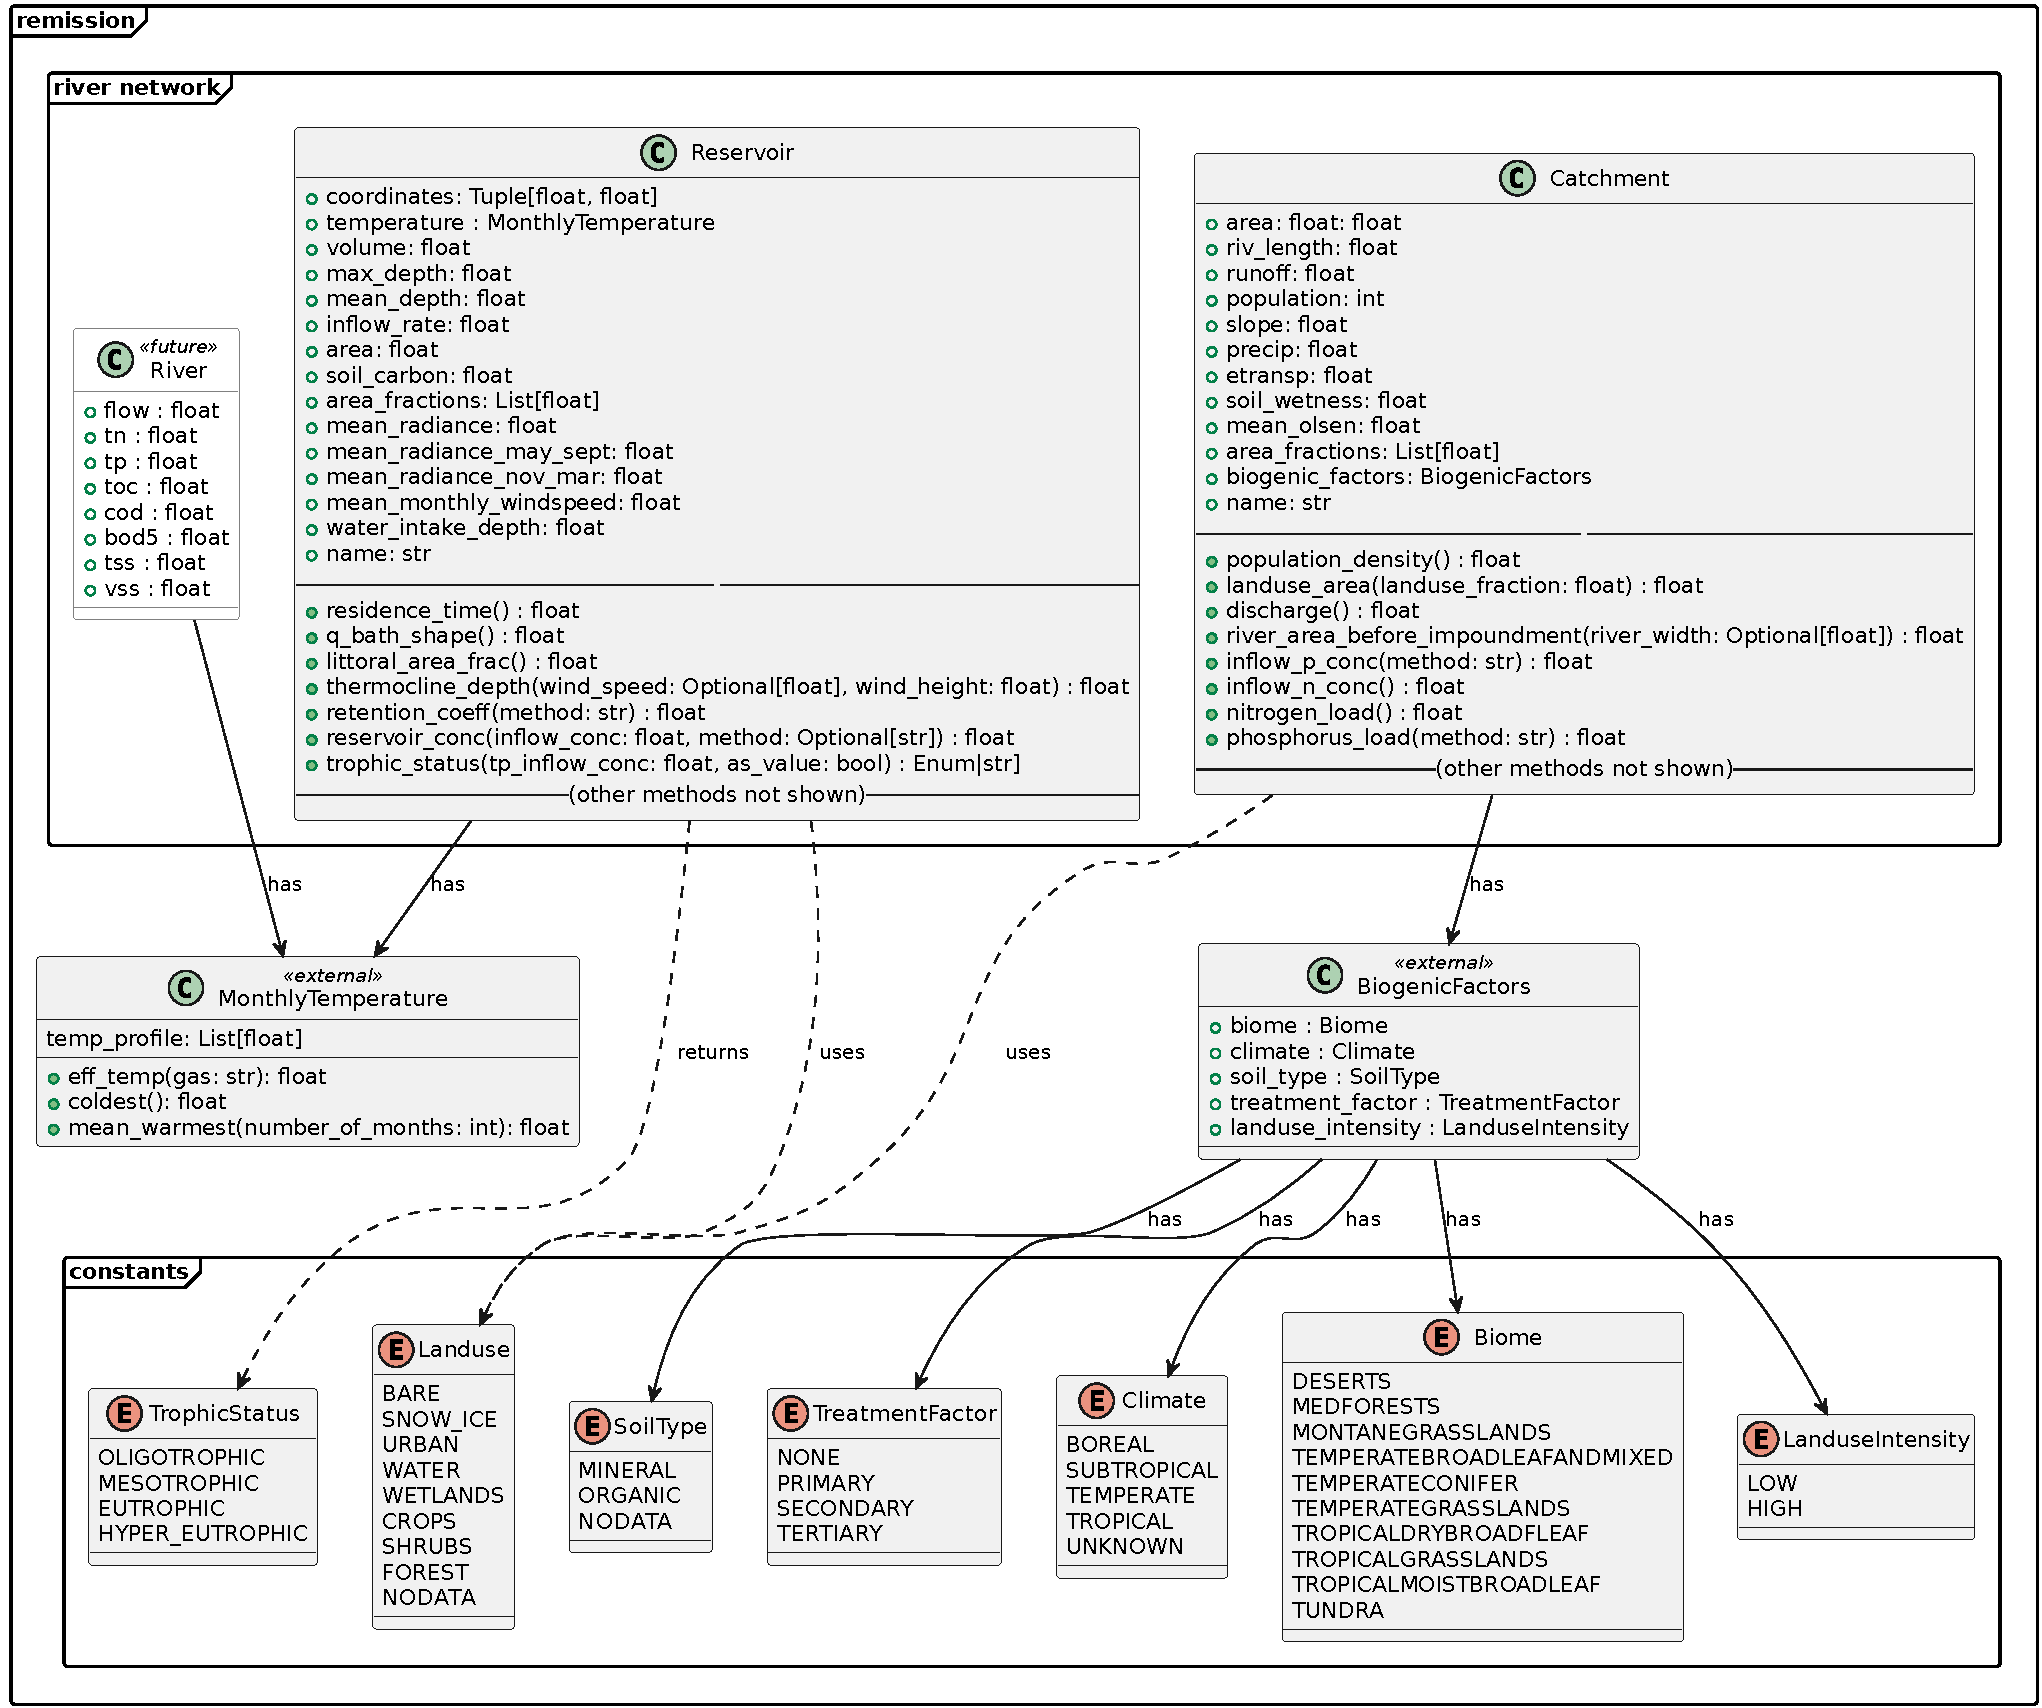
\includegraphics[width=0.99\textwidth]{figures/river_network_uml.pdf}
    \caption{A UML class diagram visualizing the \vrbbrk{Reservoir} and \vrbbrk{Catchment} classes and different container classes and categorical data representations using Enum classes.}
    \label{fig:river_network_emissions_uml}
\end{figure}

\begin{figure}[ht]
    \centering
    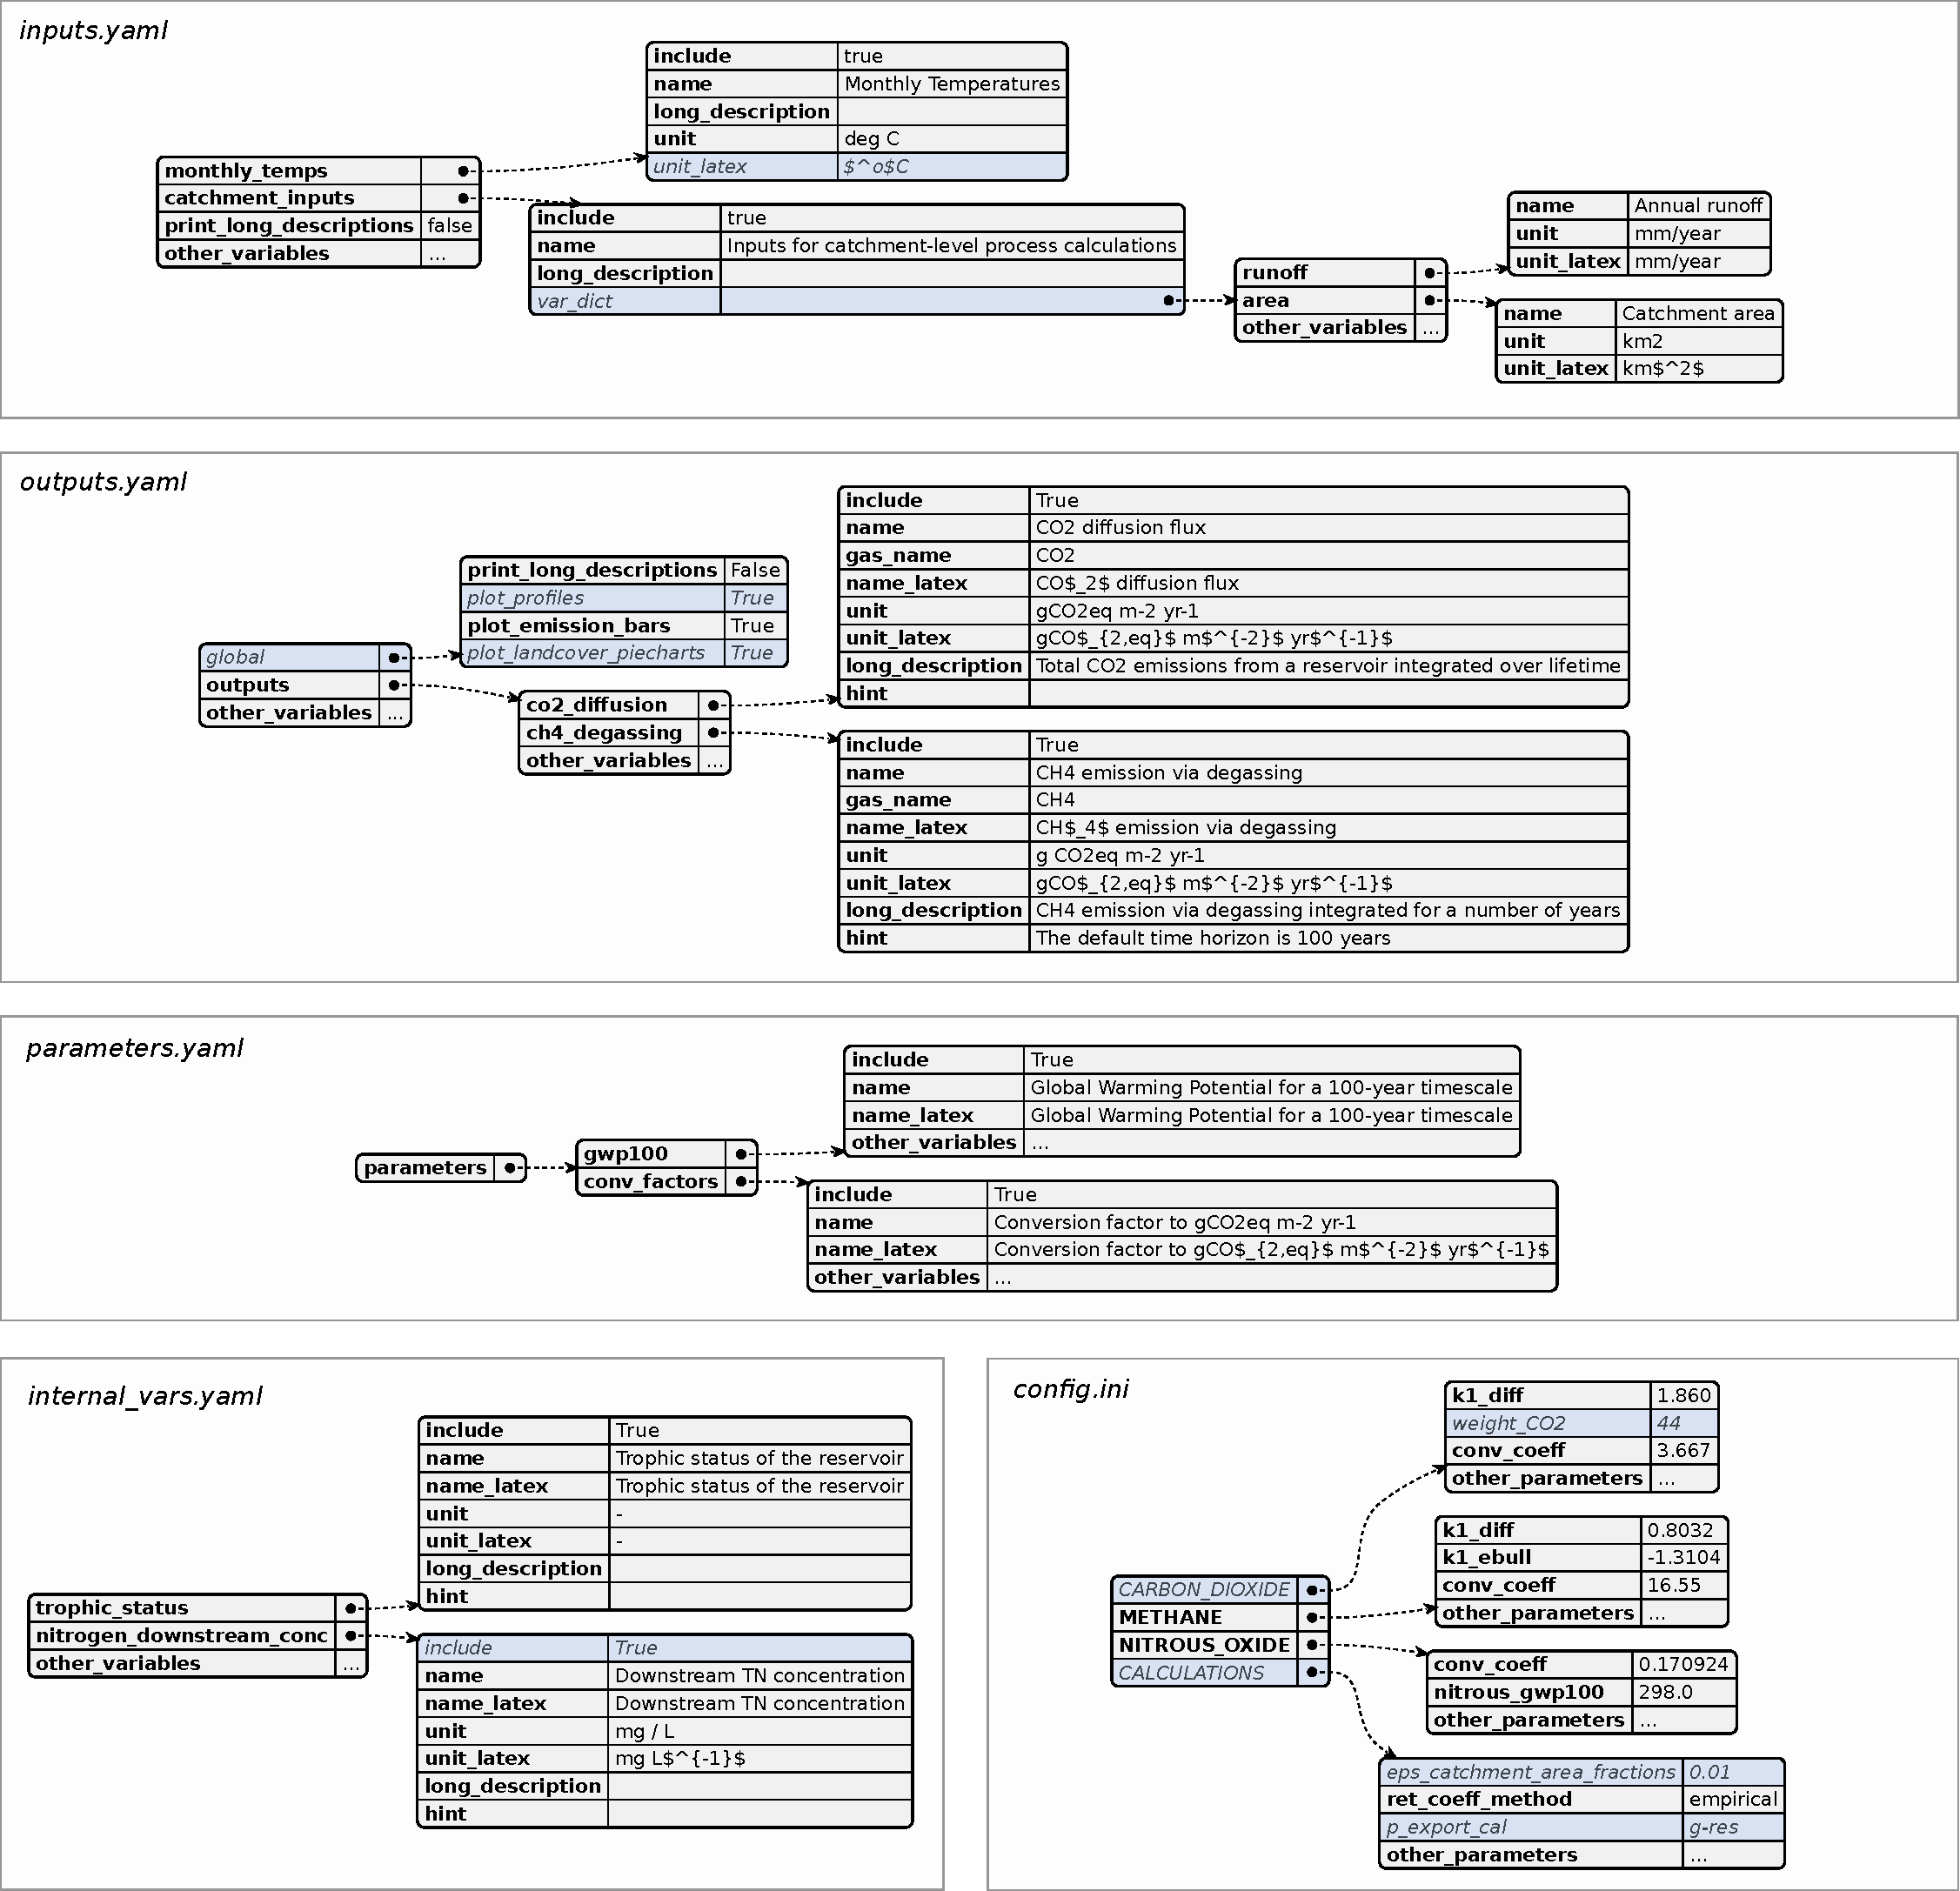
\includegraphics[width=0.99\textwidth]{figures/config_uml_portrait.pdf}
    \caption{Diagrams illustrating the structure of YAML configuration files used by the Presenter class (\vrbbrk{inputs.yaml}, \vrbbrk{outputs.yaml}, \vrbbrk{parameters.yaml}, \vrbbrk{internal\_vars.yaml}), along with the \vrbbrk{config.ini} file specifying emission model parameters and selection of alternative models.}
    \label{fig:config_uml}
\end{figure}

\begin{figure}[ht]
    \centering
    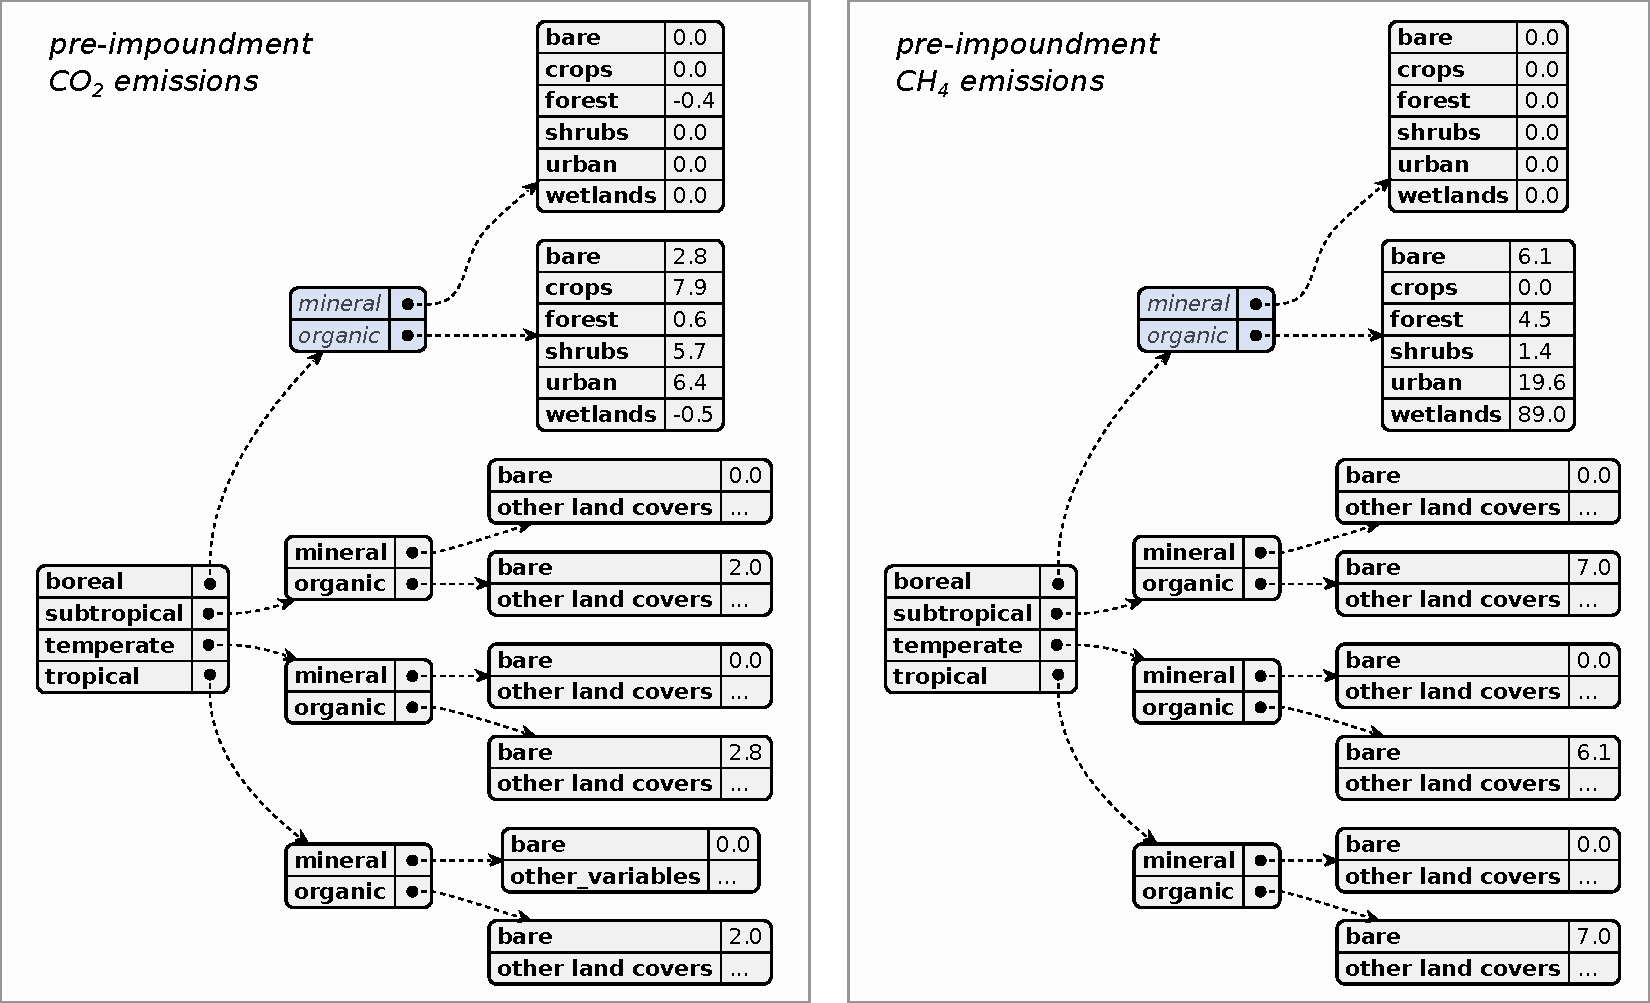
\includegraphics[width=0.80\textwidth]{figures/preimpoundment.pdf}
    \caption{Diagrams illustrating the structure of YAML configuration files and the underlying data relating areal pre-impoundment CO$_2$ and CH$_4$ emissions to climate, soil type, and land cover type.}
    \label{fig:preimpoundment}
\end{figure}

\begin{figure}[ht]
    \centering
    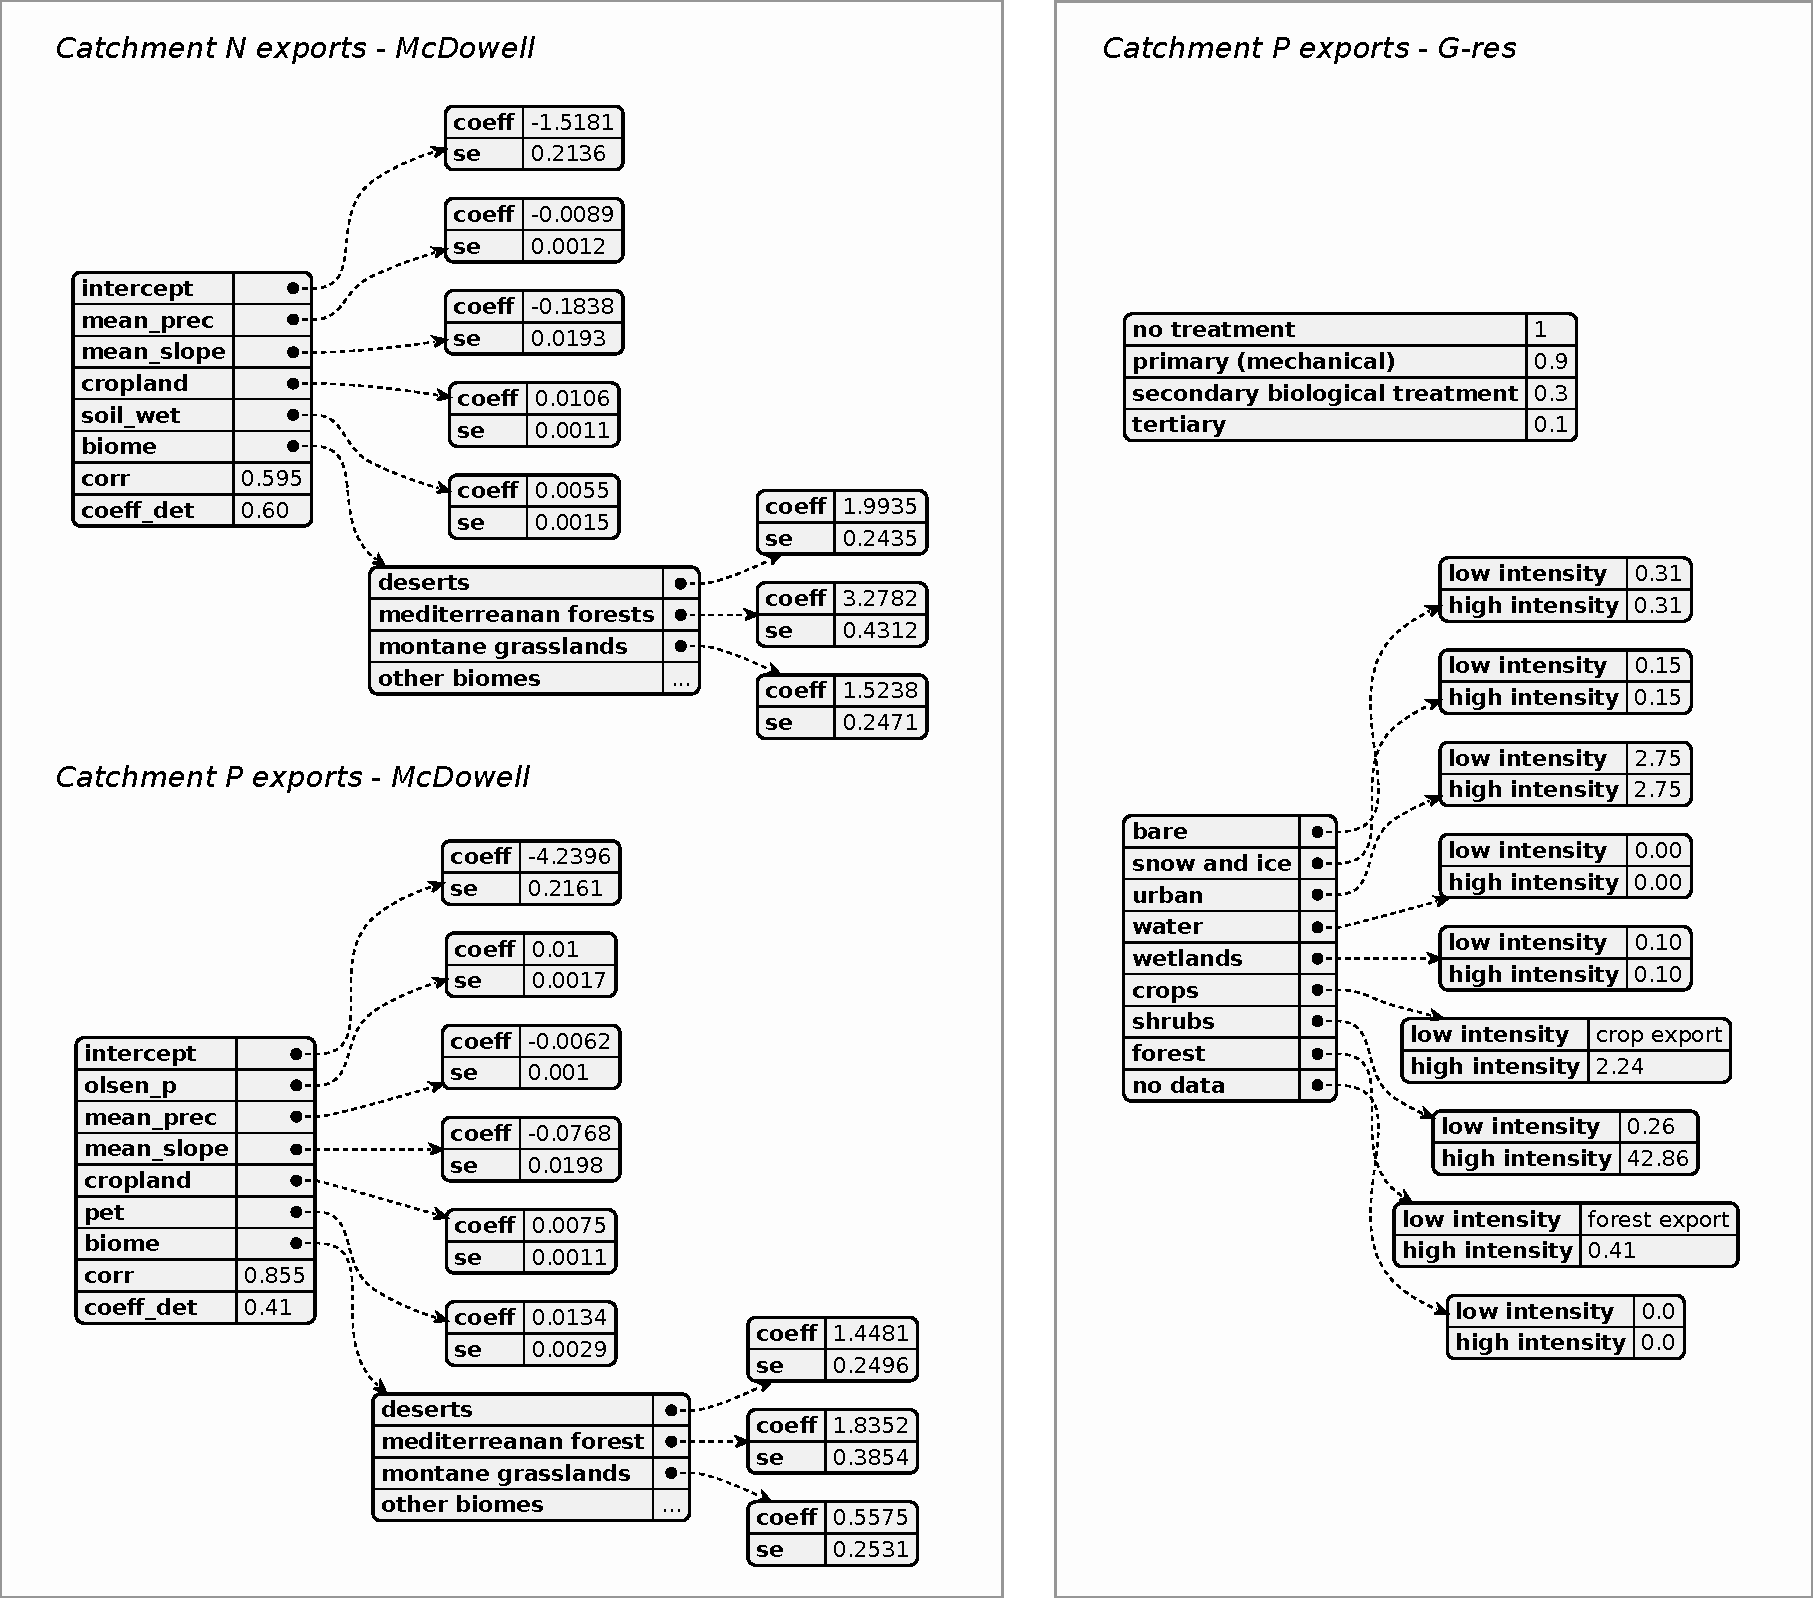
\includegraphics[width=0.85\textwidth]{figures/tp_tn_exports.pdf}
    \caption{Diagrams illustrating the structure of YAML configuration files parameterizing the nutrient export models of \citet{McDowell2020} (\ac{N} and \ac{P}) and G-res (\ac{P}).}
    \label{fig:tp_tn_exports}
\end{figure}

\begin{table}[ht]
\begin{threeparttable}
    \label{app_table:input_variables}
	{\small
    \caption{Input variables used by Re-Emission for estimating \ac{GHG} emissions from reservoirs. Additional details on the geospatial data sources used to derive these inputs are provided in Supplementary Tables 4 and 5 in \citet{janus2025planning}.}
    \label{app_table:input_variables}%
    \begin{tabular*}{\linewidth}{@{\extracolsep{\fill}}lcc@{}}
    \toprule
    Input Name & Unit & Model\tnote{2} \\
    \midrule%
    \multicolumn{3}{c}{Inputs for catchment{-}level calculations}\\%
    %\midrule%
    Biome&{-} & McDowell\tnote{3}\\%
    Climate&{-} & G-res\\%
    Soil Type&{-} & -\tnote{4}\\%
    Treatment Factor&{-} & G-res\\%
    Landuse Intensity&{-} & G-res\\%
    Monthly Temperatures&$^o$C & G-res\\%
    Annual runoff&mm/year & G-res\\%
    Catchment area&km$^2$ & G-res\\%
    Length of inundated river&km & G-res\\%
    Population&capita & G-res\\%
    Area fractions\tnote{1}&--& G-res, McDowell\tnote{3}\\%
    Mean catchment slope&\%& McDowell\tnote{3}\\%
    Mean annual precipitation&mm/year& McDowell\tnote{3}\\%
    Mean annual evapotranspiration&mm/year& McDowell\tnote{3}\\%
    Soil wetness&mm over profile& McDowell\tnote{3}\\%
    Soil Olsen P content&kgP ha$^{-1}$& McDowell\tnote{3}\\%
    \midrule%
    \multicolumn{3}{c}{Inputs for reservoir{-}level calculations}\\%
    %\midrule%
    Reservoir volume&m$^3$& G-res\\%
    Reservoir area&km$^2$& G-res\\%
    Maximum reservoir depth&m& G-res\\%
    Mean reservoir depth&m& G-res\\%
    Inundated area fractions\tnote{1}&-& G-res\\%
    Soil carbon in inundated area&kgC m$^{-2}$& G-res\\%
    Mean monthly horizontal radiance&kWh m$^{-2}$ d$^{-1}$& G-res\\%
    Mean monthly horizontal radiance: May {-} Sept&kWh m$^{-2}$ d$^{-1}$& G-res\\%
    Mean monthly horizontal radiance: Nov {-} Mar&kWh m$^{-2}$ d$^{-1}$& G-res\\%
    Mean monthly wind speed&m s$^{-1}$& G-res\\%
    Water intake depth below surface&m& G-res\\
    \bottomrule
    \end{tabular*}
    }
    {\noindent
    \begin{tablenotes}
        \footnotesize
        \item{1} Fractions of land cover in the delineated area.
        \item{2} Model implementations relying on the input variable.
        \item{3} Land nitrogen (N) and phosphorus (P) export model by McDowell et al.~\cite{McDowell2020}. P exports can serve as an alternative estimate of total P load for the G-res model, while nitrogen exports are used to inform nitrous oxide (N$_2$O) emission models.
        \item{4} Included for informational purposes only and not used as a predictive input in any of the implemented models.
    \end{tablenotes}
    }
\end{threeparttable}
\end{table}

%\FloatBarrier

\begin{acronym}
	\acro{ASEAN}{Association of Southeast Asian Nations}
	\acro{BRT}{Boosted Regression Tree}
	\acro{CO2}[CO$_2$]{carbon dioxide}
	\acro{CH4}[CH$_4$]{methane}
	\acro{CI}{continuous integration}
	%\acro{CI}{carbon intensity}
	\acro{CLI}{command line interface}
	\acro{DEM}{digital elevation model}
	\acro{DFS}{depth-first search}
	\acro{DOC}{dissolved organic carbon}
	\acro{DOF}{degree of fragmentation}
	\acro{DOR}{degree of regulation}
	\acro{EF}{emission factor}
	\acro{EFDC}{Environmental Fluid Dynamics Code}
	\acro{EI}{emission intensity}
	\acro{EPA}{U.S. Environmental Protection Agency}
	\acro{ET}{evapotranspiration}
	\acro{FHReD}{High-Resolution Global Database of Dams}
	\acro{FSL}{full supply level}
	\acro{GDrive}{Google Drive}
	\acro{GGRP}{Greenhouse Gas Reporting Program}
	\acro{GEE}{Google Earth Engine}
	\acro{GHCR}{GitHub Container Registry}
    \acro{GHG}{greenhouse gas}    
	\acro{GIS}{geographical information system}
	\acro{G-res}{GHG Reservoir Tool}
	\acro{GOOD2}{Global geOreferenced Database of Dams}
	\acro{GW}{gigawatts}
	\acro{HP}{hydropower}
	\acro{ICOLD}{International Commission on Large Dams}
	\acro{IHA}{International Hydropower Association}
	\acro{IRR}{irrigation}
	\acro{KDE}{kernel density estimate}
	\acro{IPCC}{Intergovernmental Panel on Climate Change}
	\acro{KNN}{K-Nearest Neighbours Regressor}
	\acro{LCA}{life-cycle assessment}
	\acro{ML}{machine-learning}
	\acro{MP}{multipurpose}
	\acro{MW}{megawatts}
	\acro{MOEA}{multiobjective evolutionary algorithm}
	\acro{MOO}{multiobjective optimization}
	\acro{N}{Nitrogen}
	\acro{N2O}[N$_2$O]{nitrous oxide}
	\acro{P}{Phosphorus}
	\acro{PD}{partial-dependence}
	\acro{PPA}{power purchase agreement}
	\acro{PV}{Photovoltaic}
	\acro{RF}{Random Forest}
	\acro{ROI}{region of interest}
	\acro{RoR}{run-of-river}
	\acro{RMSE}{root-mean-square-error}
	\acro{SA}{sensitivity analysis}
	\acro{SDG}{sustainable development goal}
	\acro{SES}{social and ecological system}
	\acro{SVR}{Support Vector Regression}
	\acro{xAI}{explainable artificial-intelligence}
	\acro{TN}{Total Nitrogen}
	\acro{TP}{Total Phosphorus}
	\acro{UAS}{Unrelated Anthropogenic Sources}
    \acro{VRE}{variable renewable energy}
	\acro{WEFE}{Water-Energy-Food-Ecosystems}
	\acro{WRT}{water residence time}
\end{acronym}

\bibliographystyle{unsrtnat}
\bibliography{reemission}

\end{document}

\endinput
%%
%% End of file `elsarticle-template-num.tex'.
